% =============================================================================
% EduSpace — PFA Report (4ème année Génie Logiciel)
% Compiles with: xelatex + biber
% =============================================================================
\documentclass[a4paper,12pt,oneside]{report}

% ── Encoding & Font ──────────────────────────────────────────────────────────
\usepackage{fontspec}
\setmainfont{Liberation Sans}  % Fallback for Calibri; swap to Calibri if available
% To use Calibri (if installed): \setmainfont{Calibri}

% ── Page geometry ────────────────────────────────────────────────────────────
\usepackage[
  a4paper,
  top=2.5cm,
  bottom=2.5cm,
  left=2.5cm,
  right=2.5cm
]{geometry}

% ── Spacing ──────────────────────────────────────────────────────────────────
\usepackage{setspace}
\onehalfspacing
\usepackage{parskip}

% ── Language ─────────────────────────────────────────────────────────────────
\usepackage{polyglossia}
\setdefaultlanguage{english}

% ── PDF Inclusion (for page de garde) ────────────────────────────────────────
\usepackage{pdfpages}

% ── Graphics & Colors ────────────────────────────────────────────────────────
\usepackage{graphicx}
\graphicspath{{images/}}
\usepackage[table,dvipsnames]{xcolor}

% ── Tables ───────────────────────────────────────────────────────────────────
\usepackage{booktabs}
\usepackage{tabularx}
\usepackage{longtable}
\usepackage{multirow}

% ── Figures & Floats ─────────────────────────────────────────────────────────
\usepackage{float}
\usepackage{caption}
\usepackage{subcaption}

% ── Lists ────────────────────────────────────────────────────────────────────
\usepackage{enumitem}

% ── TikZ & Gantt ─────────────────────────────────────────────────────────────
\usepackage{tikz}
\usetikzlibrary{shapes.geometric, arrows.meta, positioning, calc, fit, backgrounds}
\usepackage{pgfgantt}

% ── Code Listings ────────────────────────────────────────────────────────────
\usepackage{listings}
\definecolor{codebg}{RGB}{248,248,248}
\definecolor{codeframe}{RGB}{200,200,200}
\definecolor{codekw}{RGB}{0,0,180}
\definecolor{codecomment}{RGB}{0,128,0}
\definecolor{codestring}{RGB}{163,21,21}
\lstdefinestyle{educode}{
  backgroundcolor=\color{codebg},
  frame=single,
  rulecolor=\color{codeframe},
  basicstyle=\ttfamily\small,
  keywordstyle=\color{codekw}\bfseries,
  commentstyle=\color{codecomment}\itshape,
  stringstyle=\color{codestring},
  numbers=left,
  numberstyle=\tiny\color{gray},
  numbersep=8pt,
  breaklines=true,
  captionpos=b,
  tabsize=2,
  showstringspaces=false
}
\lstset{style=educode}

% ── Headers & Footers ────────────────────────────────────────────────────────
\usepackage{fancyhdr}
\pagestyle{fancy}
\fancyhf{}
\fancyhead[L]{\leftmark}
\fancyfoot[L]{\small PFA -- 4\textsuperscript{th} Year GL}
\fancyfoot[R]{\thepage}
\renewcommand{\headrulewidth}{0.4pt}
\renewcommand{\footrulewidth}{0.4pt}

% Plain style for chapter opening pages
\fancypagestyle{plain}{
  \fancyhf{}
  \fancyfoot[L]{\small PFA -- 4\textsuperscript{th} Year GL}
  \fancyfoot[R]{\thepage}
  \renewcommand{\headrulewidth}{0pt}
  \renewcommand{\footrulewidth}{0.4pt}
}

% ── Section Formatting ───────────────────────────────────────────────────────
\usepackage{titlesec}

\titleformat{\chapter}[display]
  {\normalfont\LARGE\bfseries}
  {\chaptertitlename\ \thechapter}{16pt}{\Huge}
\titlespacing*{\chapter}{0pt}{-20pt}{30pt}

% ── Table of Contents Formatting ─────────────────────────────────────────────
\usepackage{tocloft}
\renewcommand{\cftchapleader}{\cftdotfill{\cftdotsep}}

% ── Bibliography ─────────────────────────────────────────────────────────────
\usepackage[
  backend=biber,
  style=numeric,
  sorting=nyt,
  urldate=long
]{biblatex}
\addbibresource{references.bib}

% ── Hyperlinks ───────────────────────────────────────────────────────────────
\usepackage{hyperref}
\hypersetup{
  colorlinks=true,
  linkcolor=RoyalBlue,
  citecolor=OliveGreen,
  urlcolor=BrickRed,
  pdfauthor={BEN HASSINE Adam, CHEBIL Adam Taieb},
  pdftitle={EduSpace: A Microservices-Based Classroom Management Platform},
  pdfsubject={PFA Report -- 4th Year Software Engineering},
  pdfkeywords={microservices, classroom management, React, Node.js, Docker}
}

% ── Custom Commands ──────────────────────────────────────────────────────────
\newcommand{\eduspace}{\textsc{EduSpace}}
\newcommand{\figref}[1]{Figure~\ref{#1}}
\newcommand{\tabref}[1]{Table~\ref{#1}}
\newcommand{\secref}[1]{Section~\ref{#1}}
\newcommand{\chapref}[1]{Chapter~\ref{#1}}

% =============================================================================
% DOCUMENT START
% =============================================================================
\begin{document}

% ── Page de Garde ────────────────────────────────────────────────────────────
% =============================================================================
% Page de Garde — Include the original PDF as-is
% Will be customized manually later
% =============================================================================
\thispagestyle{empty}

\includepdf[pages=1]{assets/page-de-garde.pdf}


% ── Front Matter (Roman numerals) ────────────────────────────────────────────
\pagenumbering{roman}
\pagestyle{plain}

% Abstract
% =============================================================================
% Abstract and Keywords
% =============================================================================
\chapter*{Abstract}
\addcontentsline{toc}{chapter}{Abstract}

This report presents \eduspace{}, a web-based classroom management platform designed and developed as an end-of-year project for the 4\textsuperscript{th}-year Software Engineering program.
Built on a microservices architecture, \eduspace{} addresses the organizational and communication shortcomings of existing platforms such as Google Classroom by providing structured content management through typed posts and chapters, integrated real-time group chat, full-text search, an assignment and grading workflow, and a real-time notification system.

The system comprises seven independent backend services (User, Class, Content, File, Communication, Notification, and Search), an API Gateway, and a React single-page application.
Each service owns its dedicated PostgreSQL database and communicates asynchronously via RabbitMQ or synchronously through REST calls.
The infrastructure is containerized using Docker Compose and includes Redis for caching and rate limiting, MinIO for S3-compatible file storage, Elasticsearch for full-text search, and NGINX as a reverse proxy.

The report covers the full software development lifecycle: requirements analysis, UML modeling, system design, and implementation details including the technology stack, security measures, and DevOps practices.

\medskip
\noindent\textbf{Keywords:} microservices, classroom management, React, Node.js, Docker, WebSocket, REST API

\newpage

% Table of Contents
\tableofcontents
\newpage

% List of Figures
\listoffigures
\newpage

% List of Tables
\listoftables
\newpage

% Acronyms
% =============================================================================
% Glossary / List of Abbreviations
% =============================================================================
\chapter*{List of Abbreviations}
\addcontentsline{toc}{chapter}{List of Abbreviations}

\begin{longtable}{@{} l p{12cm} @{}}
\toprule
\textbf{Abbreviation} & \textbf{Definition} \\
\midrule
\endfirsthead
\toprule
\textbf{Abbreviation} & \textbf{Definition} \\
\midrule
\endhead
\bottomrule
\endfoot
API     & Application Programming Interface \\
CRUD    & Create, Read, Update, Delete \\
CSS     & Cascading Style Sheets \\
DB      & Database \\
DTO     & Data Transfer Object \\
HTML    & HyperText Markup Language \\
HTTP    & HyperText Transfer Protocol \\
IDE     & Integrated Development Environment \\
JSON    & JavaScript Object Notation \\
JWT     & JSON Web Token \\
MVC     & Model--View--Controller \\
ORM     & Object-Relational Mapping \\
PFA     & Projet de Fin d'Année (End-of-Year Project) \\
REST    & Representational State Transfer \\
S3      & Simple Storage Service \\
SDK     & Software Development Kit \\
SGBD    & Système de Gestion de Base de Données (DBMS) \\
SPA     & Single-Page Application \\
SQL     & Structured Query Language \\
SSL/TLS & Secure Sockets Layer / Transport Layer Security \\
UI      & User Interface \\
UML     & Unified Modeling Language \\
URL     & Uniform Resource Locator \\
UUID    & Universally Unique Identifier \\
UX      & User Experience \\
\end{longtable}

\newpage

% ── Main Matter (Arabic numerals from 1) ─────────────────────────────────────
\cleardoublepage
\pagenumbering{arabic}
\pagestyle{fancy}

% General Introduction
% =============================================================================
% General Introduction
% =============================================================================
\chapter*{General Introduction}
\addcontentsline{toc}{chapter}{General Introduction}
\markboth{General Introduction}{}

The digital transformation of education has accelerated considerably in recent years, driven by the widespread adoption of online learning tools and the growing expectations of both educators and students for seamless, technology-mediated collaboration.
Platforms such as Google Classroom, Moodle, and Microsoft Teams for Education have become essential components of modern academic environments.

However, despite their broad adoption, these platforms exhibit significant organizational and communicational shortcomings.
Course materials are often presented as flat, unsorted feeds that become difficult to navigate as content accumulates.
Communication channels between students and instructors are either absent or limited, and no dedicated in-platform space exists for peer-to-peer student collaboration.
Consequently, students frequently resort to external social media applications for group discussions---introducing distractions, fragmenting the learning experience, and excluding those who may not use a particular social network.

This report presents \eduspace{}, a web-based classroom management platform designed to address these gaps.
\eduspace{} structures study materials by type and chapter, integrates real-time group chat directly within each classroom, provides full-text search across all content, and supports a complete grading workflow.
The platform is architected as a microservices system.

\medskip
\noindent\textbf{Report structure.}\quad
The remainder of this report is organized as follows:

\begin{itemize}[nosep]
  \item \chapref{chap:presentation} provides the general context, objectives, development methodology, and a comparative study of existing solutions.
  \item \chapref{chap:requirements} details the requirements analysis, including actor identification, functional and non-functional requirements, and UML modeling.
  \item \chapref{chap:design} describes the system design, covering the architectural paradigm, the overall architecture, and object-oriented design artifacts.
  \item \chapref{chap:implementation} presents the implementation and deployment, including the technology stack, DevOps practices, security measures, and the user interfaces.
\end{itemize}

The report concludes with a summary of results, challenges encountered, and perspectives for future improvements.


% Chapter 1: General Project Presentation
% =============================================================================
% Chapter 1: General Project Presentation  (6–8 pages target)
% =============================================================================
\chapter{General Project Presentation}
\label{chap:presentation}

\section*{Introduction}

This chapter introduces the overall context and motivation behind the \eduspace{} project.
It begins by describing the problem domain---the shortcomings of current classroom management platforms---and states the specific objectives that the project seeks to achieve.
It then explains how the team organized its work, the development methodology adopted, and concludes with a comparative study of existing solutions to justify the design decisions made.

% ─────────────────────────────────────────────────────────────────────────────
\section{Context and Problem Statement}
\label{sec:context}

The digitization of higher education has progressed substantially over the past decade.
Learning Management Systems (LMS) and classroom management platforms have become indispensable tools for organizing course materials, distributing assignments, tracking student progress, and facilitating communication between instructors and learners.
Platforms such as Google Classroom~\cite{googleclassroom2024}, Moodle~\cite{moodle2024}, and Microsoft Teams for Education~\cite{msteams2024edu} are now deployed at scale across universities worldwide.

Despite their widespread adoption, these tools exhibit recurring limitations that hinder the learning experience:

\begin{enumerate}[label=(\roman*)]
  \item \textbf{Poor content organization.}
        In platforms like Google Classroom, all course materials---lectures, exercises, lab instructions, summaries---are displayed on a single, flat feed sorted by date.
        As the volume of content grows, students find it increasingly difficult to locate specific resources.
        There is no categorization by type (lecture vs.\ lab vs.\ exercise) or by chapter, and no dedicated search functionality within a classroom.

  \item \textbf{Limited communication channels.}
        Most platforms lack a built-in, dedicated space for student-to-student interaction.
        While some offer comment threads on posts, they do not provide real-time group chat.
        As a result, students typically create informal groups on external social media applications (e.g., Facebook Messenger, WhatsApp, Telegram), which introduces distractions, fragments the learning workflow, and excludes students who do not use a particular network.

  \item \textbf{Rigid classroom models.}
        Existing platforms assume a single classroom paradigm---typically a formal teacher--student hierarchy.
        They do not natively support informal or peer-led study groups where grading is irrelevant and all participants share equal standing.

  \item \textbf{Lack of advanced search.}
        Full-text search across post titles, descriptions, and attachment file names within a specific classroom is absent in most platforms, forcing users to scroll through chronological feeds manually.
\end{enumerate}

These shortcomings motivated the design of \eduspace{}: a classroom management platform that specifically targets content organization, in-platform real-time communication, flexible classroom types, and full-text search.

% ─────────────────────────────────────────────────────────────────────────────
\section{Specific Project Objectives}
\label{sec:objectives}

The primary goal of this project is to design, develop, and deploy a fully functional web-based classroom management platform that improves upon existing solutions in terms of organization, communication, and flexibility.
The specific objectives are:

\begin{enumerate}[label=\textbf{O\arabic*.}]
  \item \textbf{Structured content management.}
        Provide a system where every post belongs to a chapter and has an explicit type (Study Material, Quiz, Question, Assignment, or Announcement).
        Study materials are further categorized into sub-types: Cours, TD (tutorial exercises), TP (lab work), and Résumé (summary).
        Users can filter and sort the classroom stream by type, sub-type, chapter, and date.

  \item \textbf{Dual classroom model.}
        Support two distinct classroom modes---\emph{Teaching} (formal, with grading) and \emph{Friendly} (informal, without grading)---while reusing the same underlying data model and role system (Admin / Member).

  \item \textbf{Integrated real-time group chat.}
        Embed a WebSocket-based group chat within each classroom, with typing indicators, online presence tracking, file sharing, and paginated message history.
        The chat can be enabled or disabled by classroom administrators.
\end{enumerate}

% ─────────────────────────────────────────────────────────────────────────────
\section{Work Organization and Task Distribution}
\label{sec:organization}

The project was carried out by a team of two developers.
Rather than assigning rigid, technology-based roles (e.g., one person responsible for the entire frontend and another for the entire backend), the team adopted a \textbf{feature-based collaboration model}.
Each team member assumed full end-to-end ownership of a given feature---designing the data model, implementing the backend logic and API endpoints, and building the corresponding frontend interface.

This approach ensured that both developers maintained a holistic understanding of the system, from database schema to user interface.
Cross-cutting concerns such as UML diagram design, shared utility development, and architectural decisions were handled collaboratively.

Source code was managed using \textbf{Git} with a remote repository hosted on \textbf{GitHub}.
Feature branches were used to isolate work on individual services or features, and changes were integrated into the main branch through pull requests, enabling peer review before merging.
This workflow provided traceability, facilitated parallel development, and minimized integration conflicts.

% ─────────────────────────────────────────────────────────────────────────────
\section{Adopted Development Approach}
\label{sec:methodology}

Given the two-person team size and the microservices nature of the project, the team adopted an \textbf{iterative and incremental} development approach rather than a prescriptive framework such as Scrum.

Work was organized by \textbf{service and feature}: each microservice was developed end-to-end in a single iteration---backend logic, API endpoints, database schema, and the corresponding frontend views.
Once a service was functional and tested in isolation, the team proceeded to the next.
Cross-service integration (event wiring, inter-service REST calls) was addressed in dedicated integration iterations.

Each service followed the same iterative cycle: database schema design, backend logic and API endpoints, frontend UI, service-level testing, and cross-service integration---before proceeding to the next service.

% ─────────────────────────────────────────────────────────────────────────────
\section{State of the Art}
\label{sec:state-of-art}

% Note: Section 1.5.1 "Collecte de l'information" is facultatif — omitted per instructions.

\subsection{Existing Solutions}
\label{sec:existing-solutions}

Before defining the feature set of \eduspace{}, an analysis of the most prominent classroom management platforms was conducted.
The three solutions examined are Google Classroom, Moodle, and Microsoft Teams for Education.

\medskip
\tabref{tab:comparison} provides a comparative summary of these platforms against the key criteria addressed by \eduspace{}.

\begin{table}[H]
  \centering
  \caption{Comparison of existing classroom management platforms.}
  \label{tab:comparison}
  \small
  \begin{tabularx}{\textwidth}{@{} l *{4}{>{\centering\arraybackslash}X} @{}}
    \toprule
    \textbf{Criterion} & \textbf{Google Classroom} & \textbf{Moodle} & \textbf{MS Teams Edu} & \textbf{EduSpace} \\
    \midrule
    Content categorization by type     & No  & Partial & No  & Yes \\
    Chapter-based organization         & No  & Yes     & No  & Yes \\
    Full-text search within classroom  & No  & Partial & No  & Yes \\
    Integrated real-time group chat    & No  & No      & Yes & Yes \\
    Dual classroom model (formal/informal) & No & No   & No  & Yes \\
    Assignment \& grading workflow     & Yes & Yes     & Yes & Yes \\
    File attachments on all post types & Yes & Yes     & Yes & Yes \\
    Real-time notifications            & Partial & No  & Yes & Yes \\
    Open-source                        & No  & Yes     & No  & Yes \\
    Lightweight deployment (Docker)    & N/A & Complex & N/A & Yes \\
    Modern, responsive UI              & Yes & No      & Yes & Yes \\
    \bottomrule
  \end{tabularx}
\end{table}

% ─────────────────────────────────────────────────────────────────────────────
\subsection{Critiques and Recommendations}
\label{sec:critiques}

The comparative analysis reveals several gaps that no single existing platform fully addresses:

\begin{enumerate}[label=(\roman*)]
  \item \textbf{Content discoverability.}
        Google Classroom and Microsoft Teams for Education both lack structured content categorization.
        While Moodle offers course sections, its interface complexity offsets this advantage.
        \emph{Recommendation:} Combine type-based and chapter-based organization with full-text search powered by a dedicated search engine.

  \item \textbf{In-platform communication.}
        Only Microsoft Teams provides real-time chat, but it is embedded within a large, general-purpose collaboration suite.
        Google Classroom and Moodle offer no real-time messaging.
        \emph{Recommendation:} Integrate a lightweight, WebSocket-based group chat directly within each classroom, with the option for administrators to enable or disable it.

  \item \textbf{Classroom flexibility.}
        All three platforms assume a single classroom paradigm.
        \emph{Recommendation:} Support both a formal (teaching) mode with full grading capabilities and an informal (friendly) mode for peer-led study groups, reusing the same underlying architecture.
  \end{enumerate}

These recommendations directly informed the design decisions and feature set of \eduspace{}, as detailed in the subsequent chapters.

% ─────────────────────────────────────────────────────────────────────────────
\section*{Conclusion}

This chapter established the context and motivation for \eduspace{} by identifying the organizational and communicational limitations of existing classroom management platforms.


The next chapter details the requirements analysis, including actor identification, functional and non-functional requirements, and UML modeling of the system's behavior.


% Chapter 2: Requirements Analysis
% =============================================================================
% Chapter 2: Requirements Analysis  (10–14 pages target)
% =============================================================================
\chapter{Requirements Analysis}
\label{chap:requirements}

\section*{Introduction}

This chapter presents a thorough analysis of the requirements that guided the design and implementation of \eduspace{}.
It begins by identifying the actors who interact with the system and defining the functional and non-functional requirements.
It then presents the UML modeling artifacts---use case diagrams, use case descriptions, and system sequence diagrams---that formalize the system's expected behavior.
The chapter concludes with the task distribution and project planning.

% =============================================================================
\section{Identification of Actors and Requirements}
\label{sec:actors-requirements}

% ─────────────────────────────────────────────────────────────────────────────
\subsection{Persona Sheets (System Actors)}
\label{sec:personas}

The \eduspace{} platform defines four actors, distinguished by their authentication state and their role within a given classroom.

\begin{enumerate}[label=\textbf{A\arabic*.}]
  \item \textbf{Visitor.}
        An unauthenticated user who can access public pages (landing page, login, registration, password reset).
        A visitor becomes a \emph{User} after registering and verifying their email address.

  \item \textbf{User (Authenticated).}
        A registered and verified individual who can access the dashboard, create or join classrooms, manage their profile, and view notifications and the calendar.
        Upon entering a classroom, the user assumes one of the two classroom-level roles below.

  \item \textbf{Member.}
        A user who has joined a classroom with the \texttt{MEMBER} role.
        Members can view the stream, filter and search posts, comment, submit assignments (in Teaching classrooms), view their own grades, and participate in the group chat.

  \item \textbf{Admin.}
        A user who holds the \texttt{ADMIN} role in a classroom (the creator is automatically an Admin; other members can be promoted).
        In addition to all Member capabilities, Admins can create, edit, and delete posts, manage chapters, manage members (promote or remove), grade submissions, configure classroom settings, and enable or disable the chat.
\end{enumerate}

% ─────────────────────────────────────────────────────────────────────────────
\subsection{Functional Requirements}
\label{sec:functional-requirements}

The functional requirements of \eduspace{} are organized below by domain.
Each requirement is derived from the project specification and describes a concrete capability that the system provides to its users.

% ── Authentication & User Management ────────────────────────────────────────
\subsubsection{Authentication and User Management}

\begin{enumerate}[label=\textbf{FR-\arabic*.}, leftmargin=2.5cm]
  \item \textbf{Registration.}
        A visitor can create an account by providing an email address, a password, a first name, and a last name.
        The password is hashed using bcrypt before storage.

  \item \textbf{Email verification.}
        Upon registration, the system sends a six-digit verification code to the provided email address.
        The user must enter this code to activate the account.

  \item \textbf{Login.}
        A registered and verified user can log in with email and password.

  \item \textbf{Password reset.}
        A user who has forgotten their password can request a reset link via email.

  \item \textbf{Profile management.}
        An authenticated user can view and update their profile information.

  \item \textbf{Account deletion.}
        An authenticated user can permanently delete their account.
\end{enumerate}

\begin{figure}[H]
  \centering
  
\includegraphics[width=0.85\textwidth]{figma/01 login.png}
  \caption{Figma mockup of the login page.}
  \label{fig:figma-login}
\end{figure}

% ── Classroom Management ────────────────────────────────────────────────────
\subsubsection{Classroom Management}

\begin{enumerate}[label=\textbf{FR-\arabic*.}, leftmargin=2.5cm, resume]
  \item \textbf{Classroom creation.}
        An authenticated user can create a classroom (\emph{Teaching} or \emph{Friendly}).
        The system generates a unique six-character alphanumeric class code.

  \item \textbf{Dual classroom model.}
        The platform supports two classroom types:
        \begin{itemize}[nosep]
          \item \emph{Teaching} --- the creator and promoted users are displayed as ``Teachers,'' joiners as ``Students.'' Grading features are fully enabled.
          \item \emph{Friendly} --- the creator and promoted users are displayed as ``Admins,'' joiners as ``Members.'' Grading features are hidden entirely; the API rejects any grading-related requests.
        \end{itemize}
        Both types use the same two internal roles: \texttt{ADMIN} and \texttt{MEMBER}.

  \item \textbf{Joining a classroom.}
        Any authenticated user can join a classroom by entering its six-character class code.

  \item \textbf{Leaving a classroom.}
        Any member (except the creator) can leave a classroom voluntarily.

  \item \textbf{Classroom settings.}
        Administrators can update the classroom name, description, section, subject, cover image, and the chat toggle (enable or disable group chat).

  \item \textbf{Classroom deletion.}
        Only the original creator of a classroom can delete it.

  \item \textbf{Listing classrooms.}
        An authenticated user can view a dashboard showing all classrooms they belong to.
\end{enumerate}

\begin{figure}[H]
  \centering
  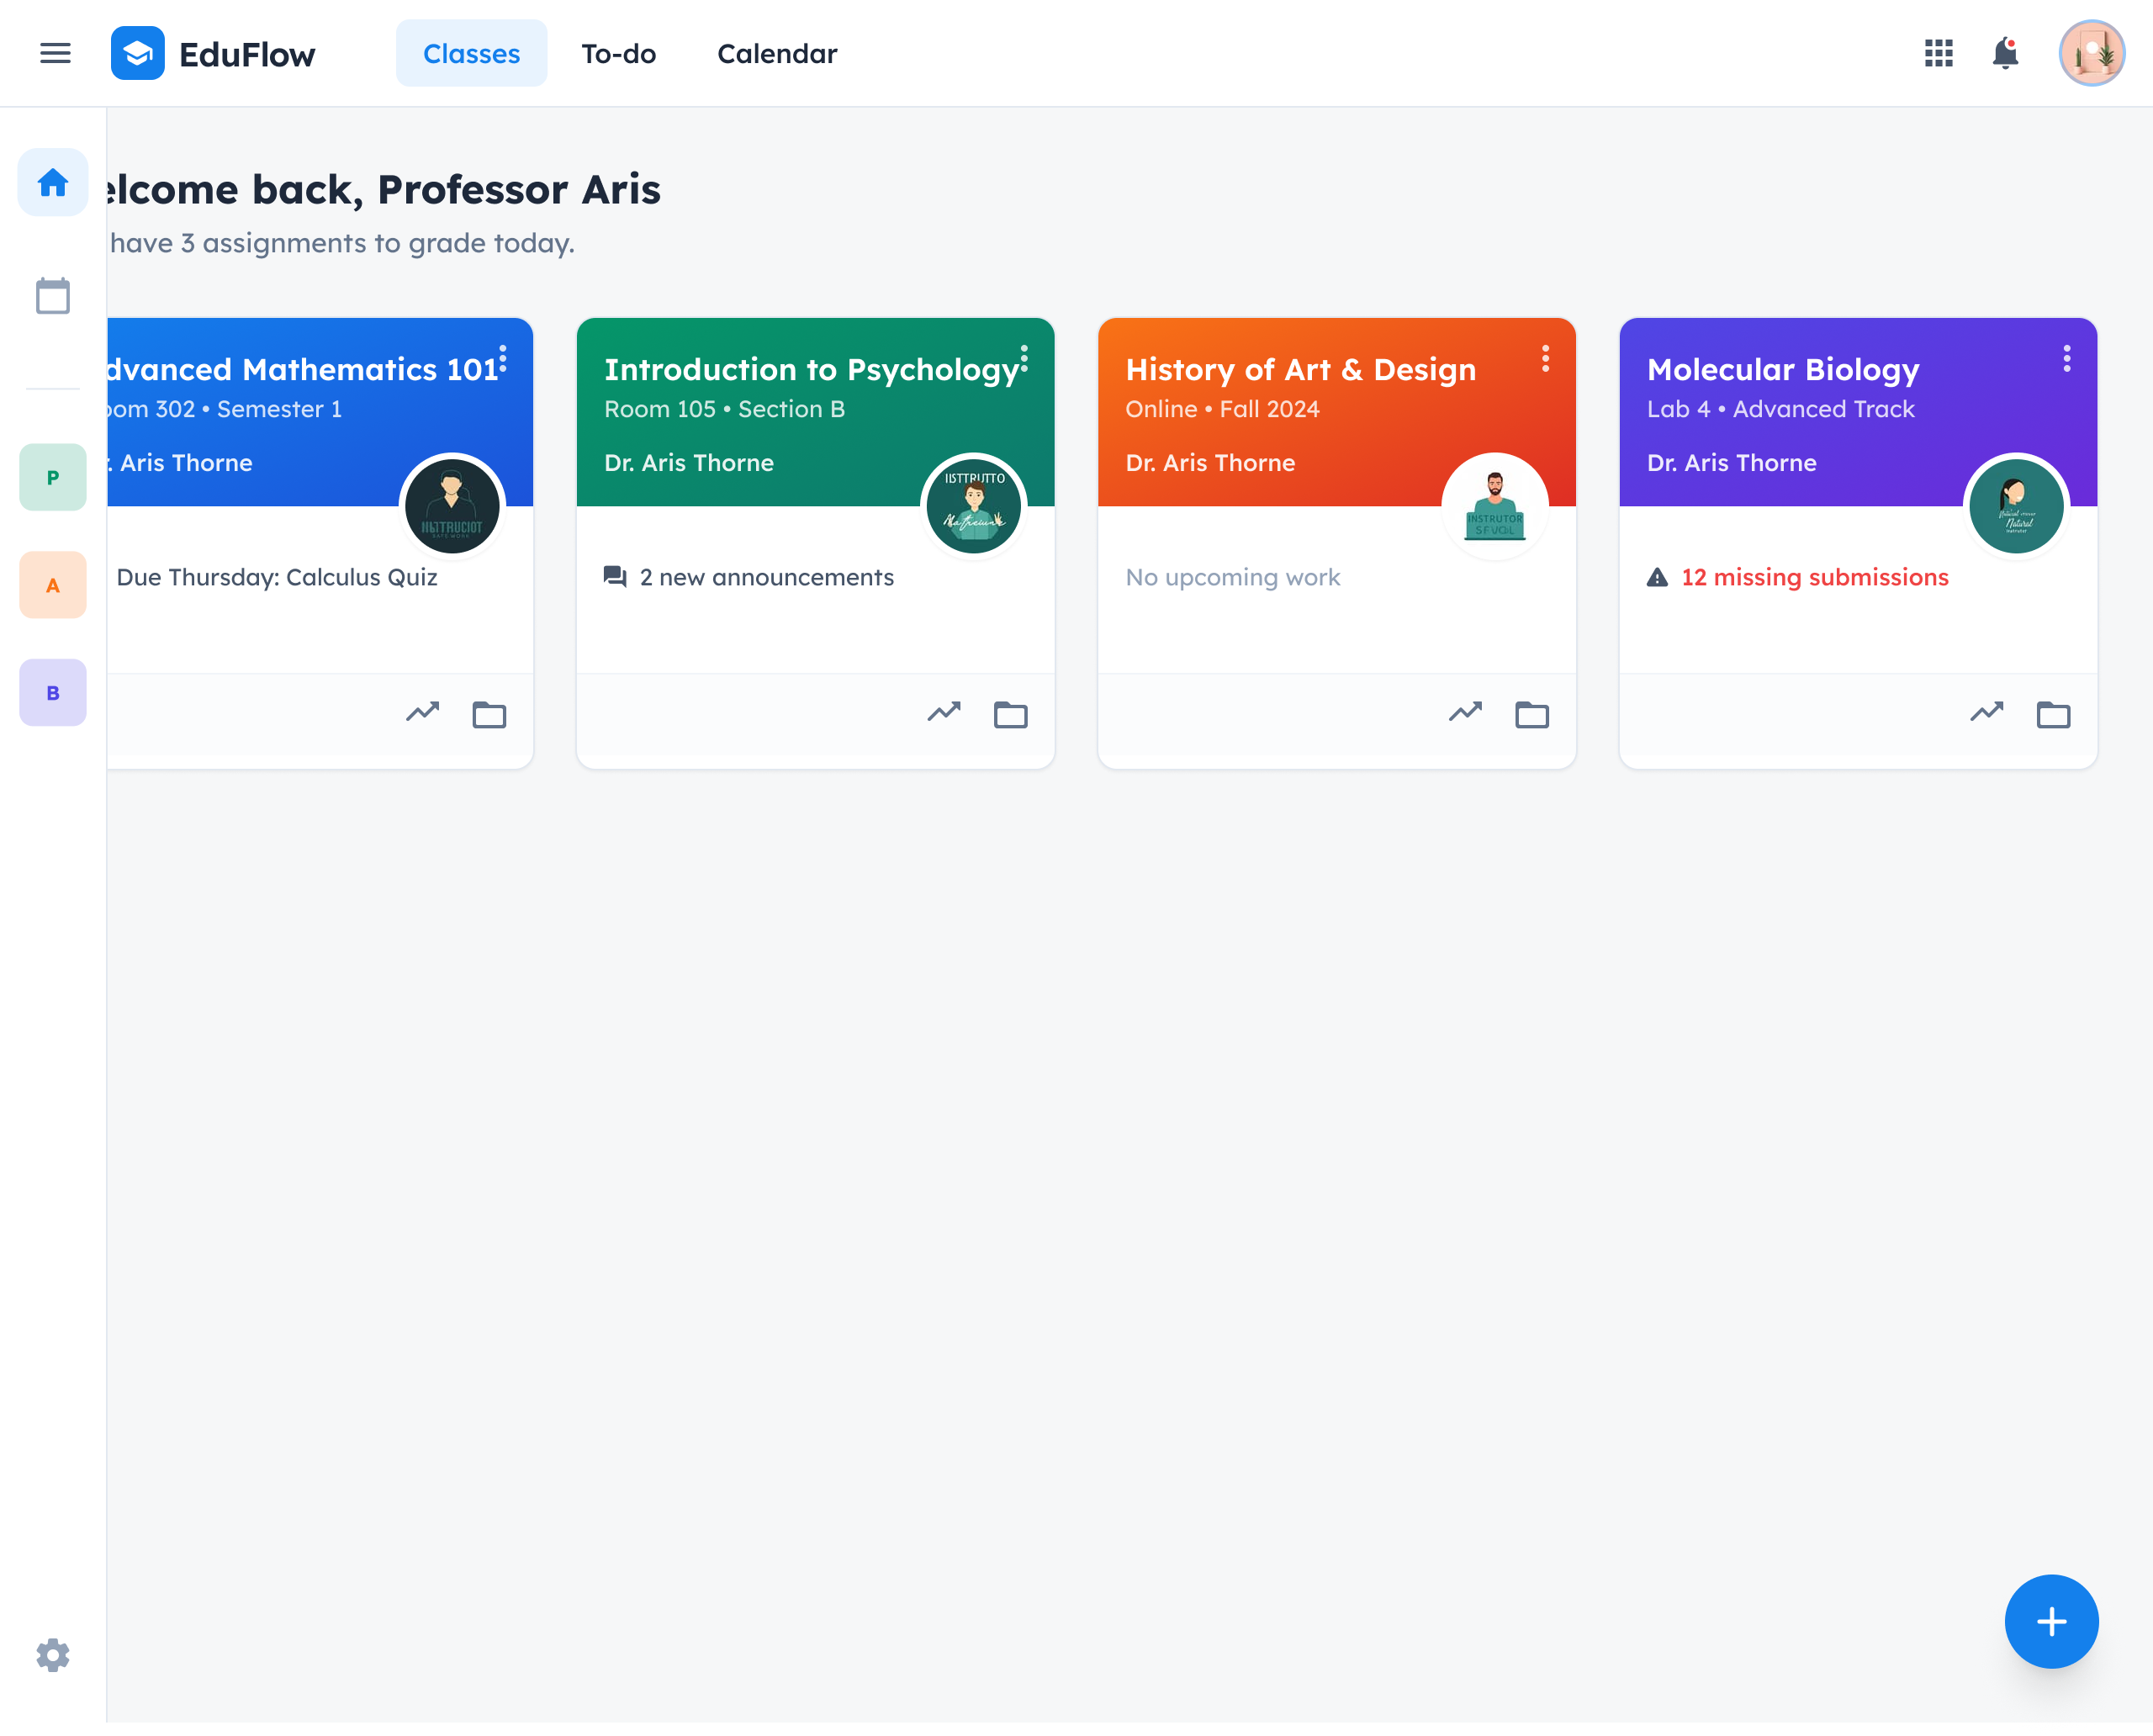
\includegraphics[width=0.85\textwidth]{figma/05 dashboard-with-classrooms.png}
  \caption{Figma mockup of the dashboard with classroom cards.}
  \label{fig:figma-dashboard}
\end{figure}

% ── Member Management ───────────────────────────────────────────────────────
\subsubsection{Member Management}

\begin{enumerate}[label=\textbf{FR-\arabic*.}, leftmargin=2.5cm, resume]
  \item \textbf{Member listing.}
        All classroom members can view the list of members, grouped by role.
        The header labels adapt to the classroom type (``Teachers \& Students'' vs.\ ``Admins \& Members'').

  \item \textbf{Role promotion.}
        An administrator can promote a \texttt{MEMBER} to \texttt{ADMIN}.

  \item \textbf{Member removal.}
        An administrator can remove any member from the classroom, except the classroom creator.
\end{enumerate}


% ── Chapter Management ──────────────────────────────────────────────────────
\subsubsection{Chapter Management}

\begin{enumerate}[label=\textbf{FR-\arabic*.}, leftmargin=2.5cm, resume]
  \item \textbf{Chapter creation.}
        Administrators can create new chapters within a classroom to organize content thematically.

  \item \textbf{Chapter reordering.}
        Administrators can reorder chapters by drag-and-drop.

  \item \textbf{Chapter editing and deletion.}
        Administrators can rename or delete chapters.
        The ``General'' chapter, which is auto-created with each classroom, cannot be renamed or deleted.
\end{enumerate}

% ── Post Management ─────────────────────────────────────────────────────────
\subsubsection{Post Management}

\begin{enumerate}[label=\textbf{FR-\arabic*.}, leftmargin=2.5cm, resume]
  \item \textbf{Post creation.}
        Administrators can create posts within a classroom.
        Each post requires a title, a type, and a chapter assignment.
        The five post types are:
        \begin{itemize}[nosep]
          \item \textbf{Study Material} --- further categorized into sub-types: Cours (lecture material), TD (tutorial exercises), TP (lab work), and Summary.
          \item \textbf{Quiz} --- a quiz or test for the class.
          \item \textbf{Question} --- a question posted to the class.
          \item \textbf{Assignment} --- includes a due date and maximum points (Teaching classrooms only).
          \item \textbf{Announcement} --- a general announcement.
        \end{itemize}
        All post types support optional text content and file attachments.

  \item \textbf{Post viewing.}
        All members can view posts.
        The \emph{Stream} tab displays posts in reverse chronological order.

  \item \textbf{Stream filtering and sorting.}
        The stream provides a toolbar with:
        \begin{itemize}[nosep]
          \item A type filter (all types, or a specific type; selecting Study Material reveals a secondary sub-type filter).
          \item A chapter filter (all chapters, or a specific chapter).
          \item Sort controls (newest first, oldest first, title A--Z, title Z--A).
          \item A search bar connected to the full-text search engine.
        \end{itemize}

  \item \textbf{Post editing and deletion.}
        Any administrator can update or delete any post in the classroom.

  \item \textbf{Commenting.}
        All members can post comments on any post.
        Comment authors can edit or delete their own comments.
        Administrators can delete any comment.
\end{enumerate}

\begin{figure}[H]
  \centering
  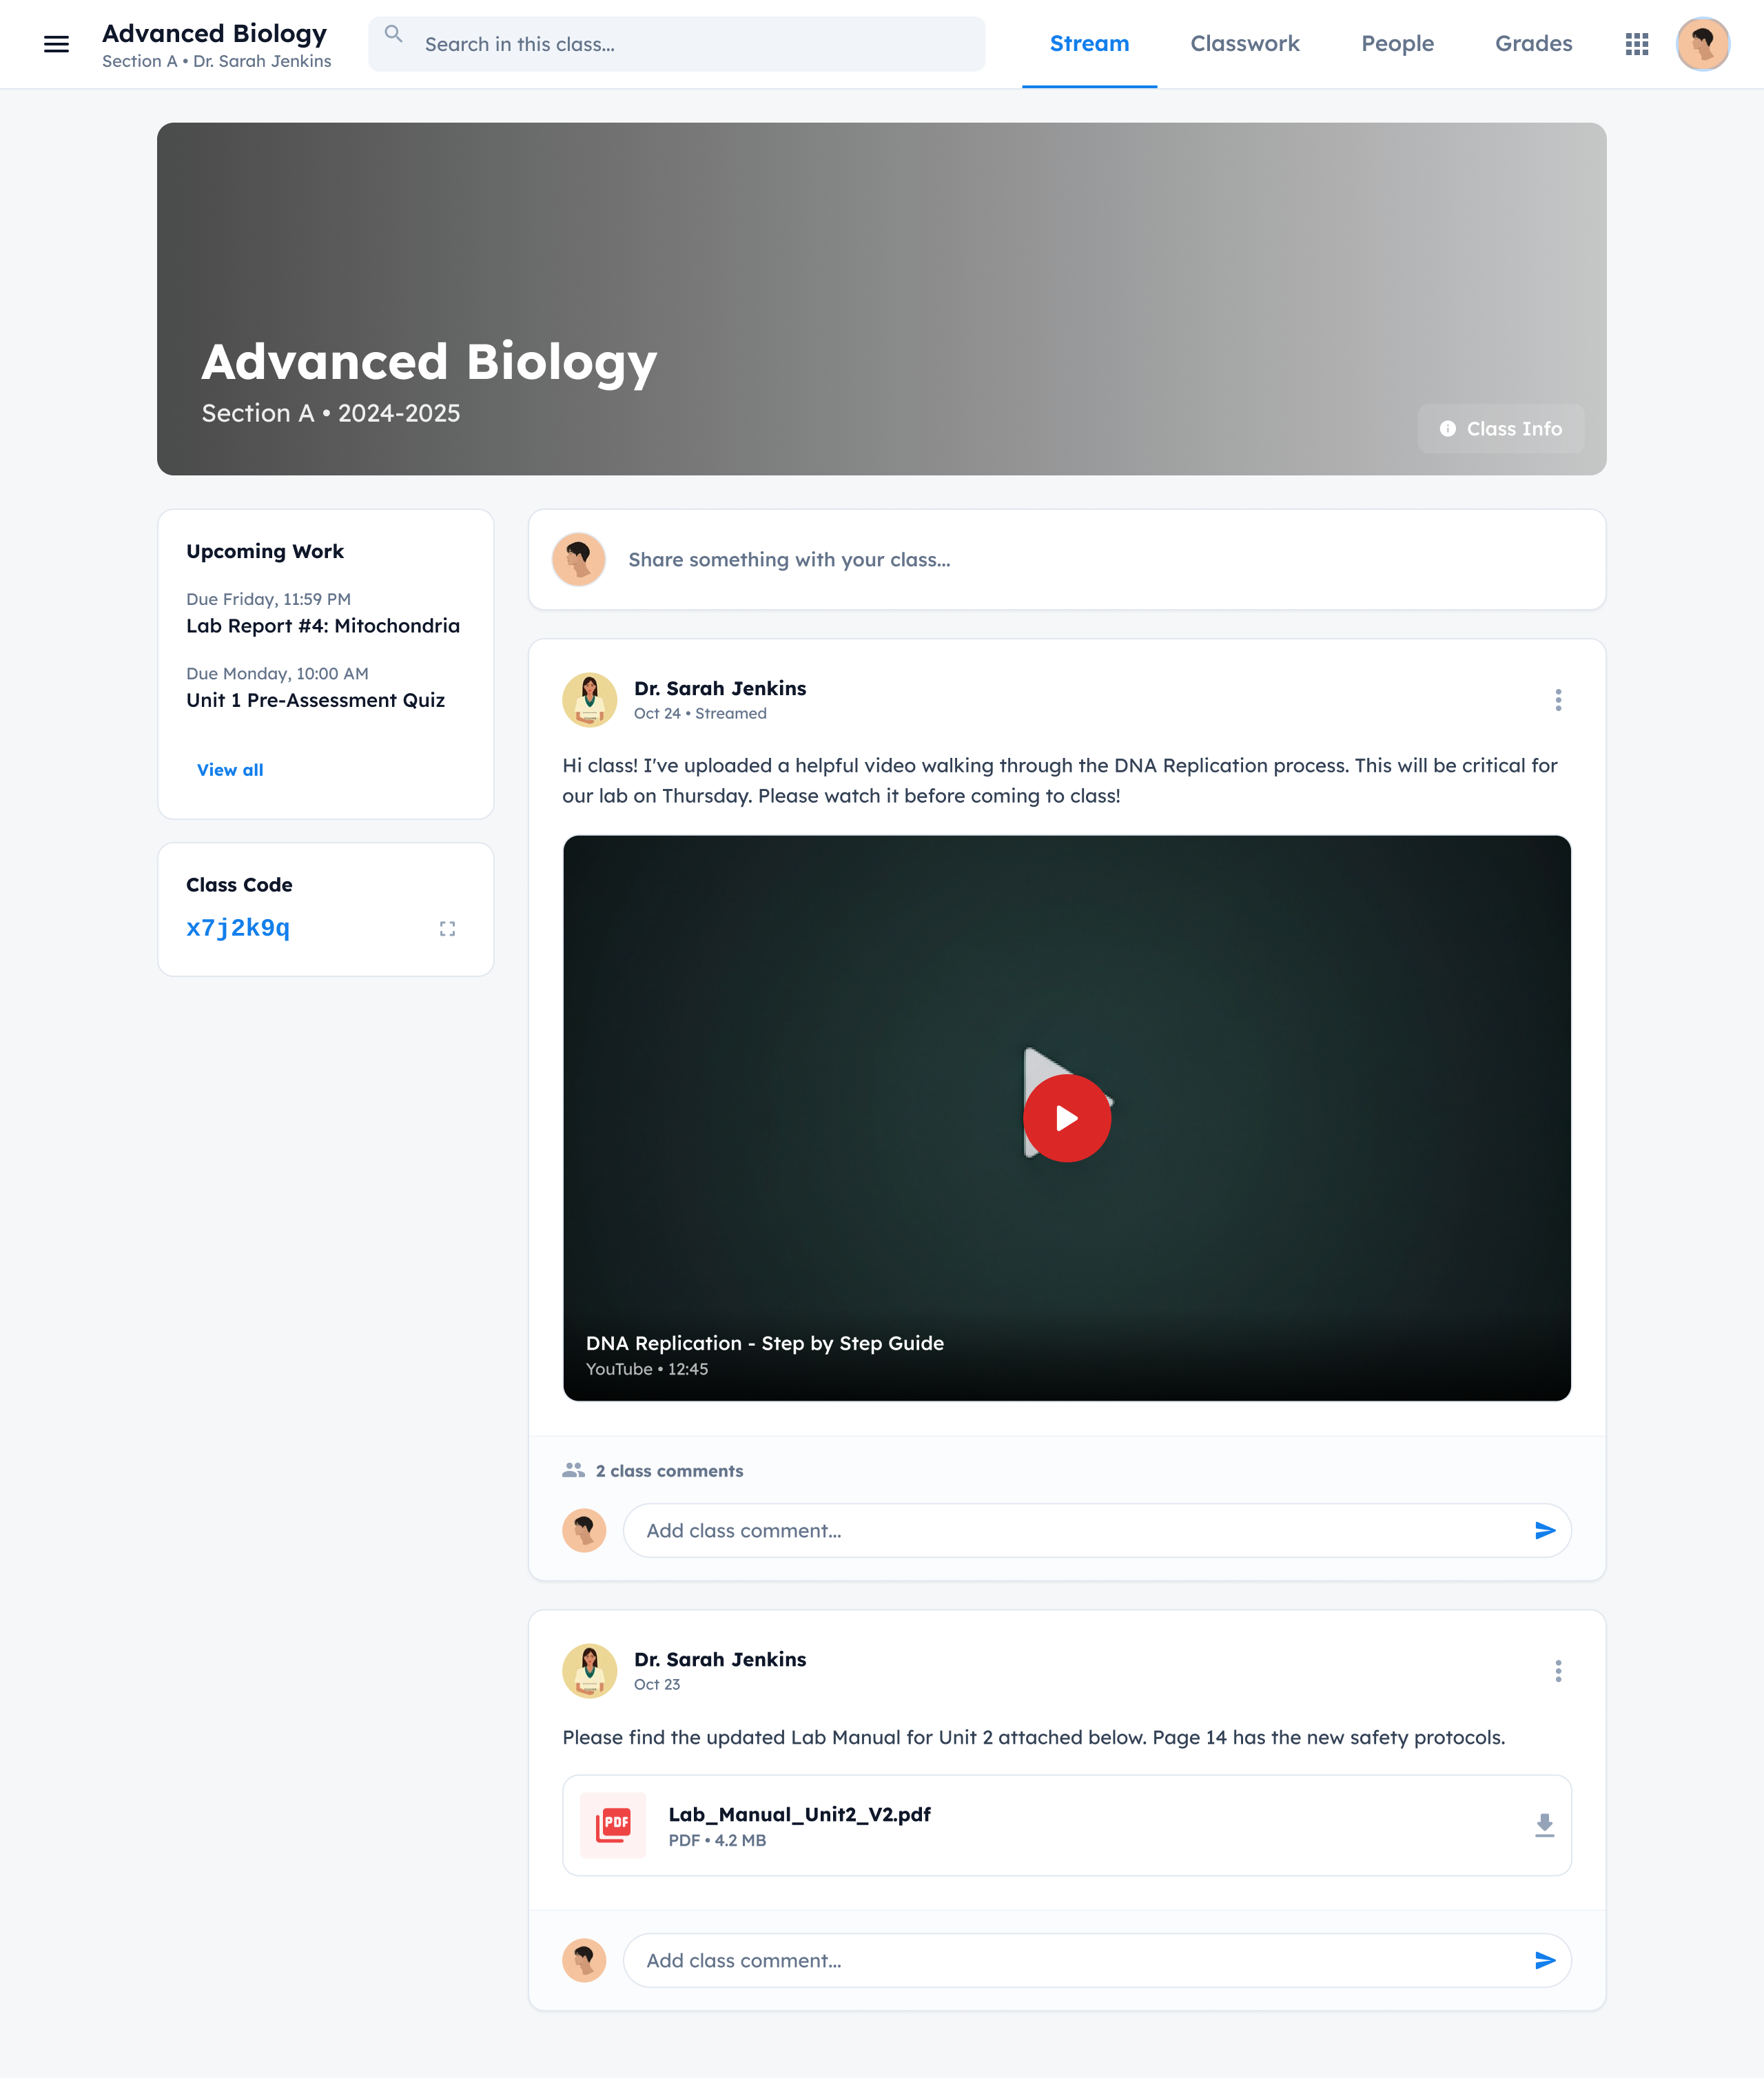
\includegraphics[width=0.85\textwidth]{figma/13 stream-tab.png}
  \caption{Figma mockup of the Stream tab with post feed and filter toolbar.}
  \label{fig:figma-stream}
\end{figure}

% ── Assignment and Grading Workflow ─────────────────────────────────────────
\subsubsection{Assignment and Grading Workflow}

These features are available exclusively in \emph{Teaching} classrooms.

\begin{enumerate}[label=\textbf{FR-\arabic*.}, leftmargin=2.5cm, resume]
  \item \textbf{Assignment submission.}
        Members can submit work for an assignment by providing optional text content and file attachments.

  \item \textbf{Submission grading.}
        Administrators can view all submissions for an assignment.

  \item \textbf{Assignments calendar.}
        A calendar view (month and week modes) displays assignment due dates for the classroom, providing a visual overview of upcoming deadlines.
\end{enumerate}


% ── Communication ───────────────────────────────────────────────────────────
\subsubsection{Real-Time Group Chat}

\begin{enumerate}[label=\textbf{FR-\arabic*.}, leftmargin=2.5cm, resume]
  \item \textbf{Automatic chat room creation.}
        When a classroom is created with chat enabled, a dedicated chat room is automatically provisioned.
        Each classroom has exactly one chat room.

  \item \textbf{Chat toggle.}
        Administrators can enable or disable the group chat via classroom settings.
        Disabling the chat hides the Chat tab from the interface but does not delete the chat history.

  \item \textbf{Real-time messaging.}
        Members can send text messages and share files in real time using WebSocket connections (Socket.IO).

  \item \textbf{Typing indicators.}
        The system broadcasts typing and stop-typing events to all connected members in the same chat room.
\end{enumerate}

\begin{figure}[H]
  \centering
  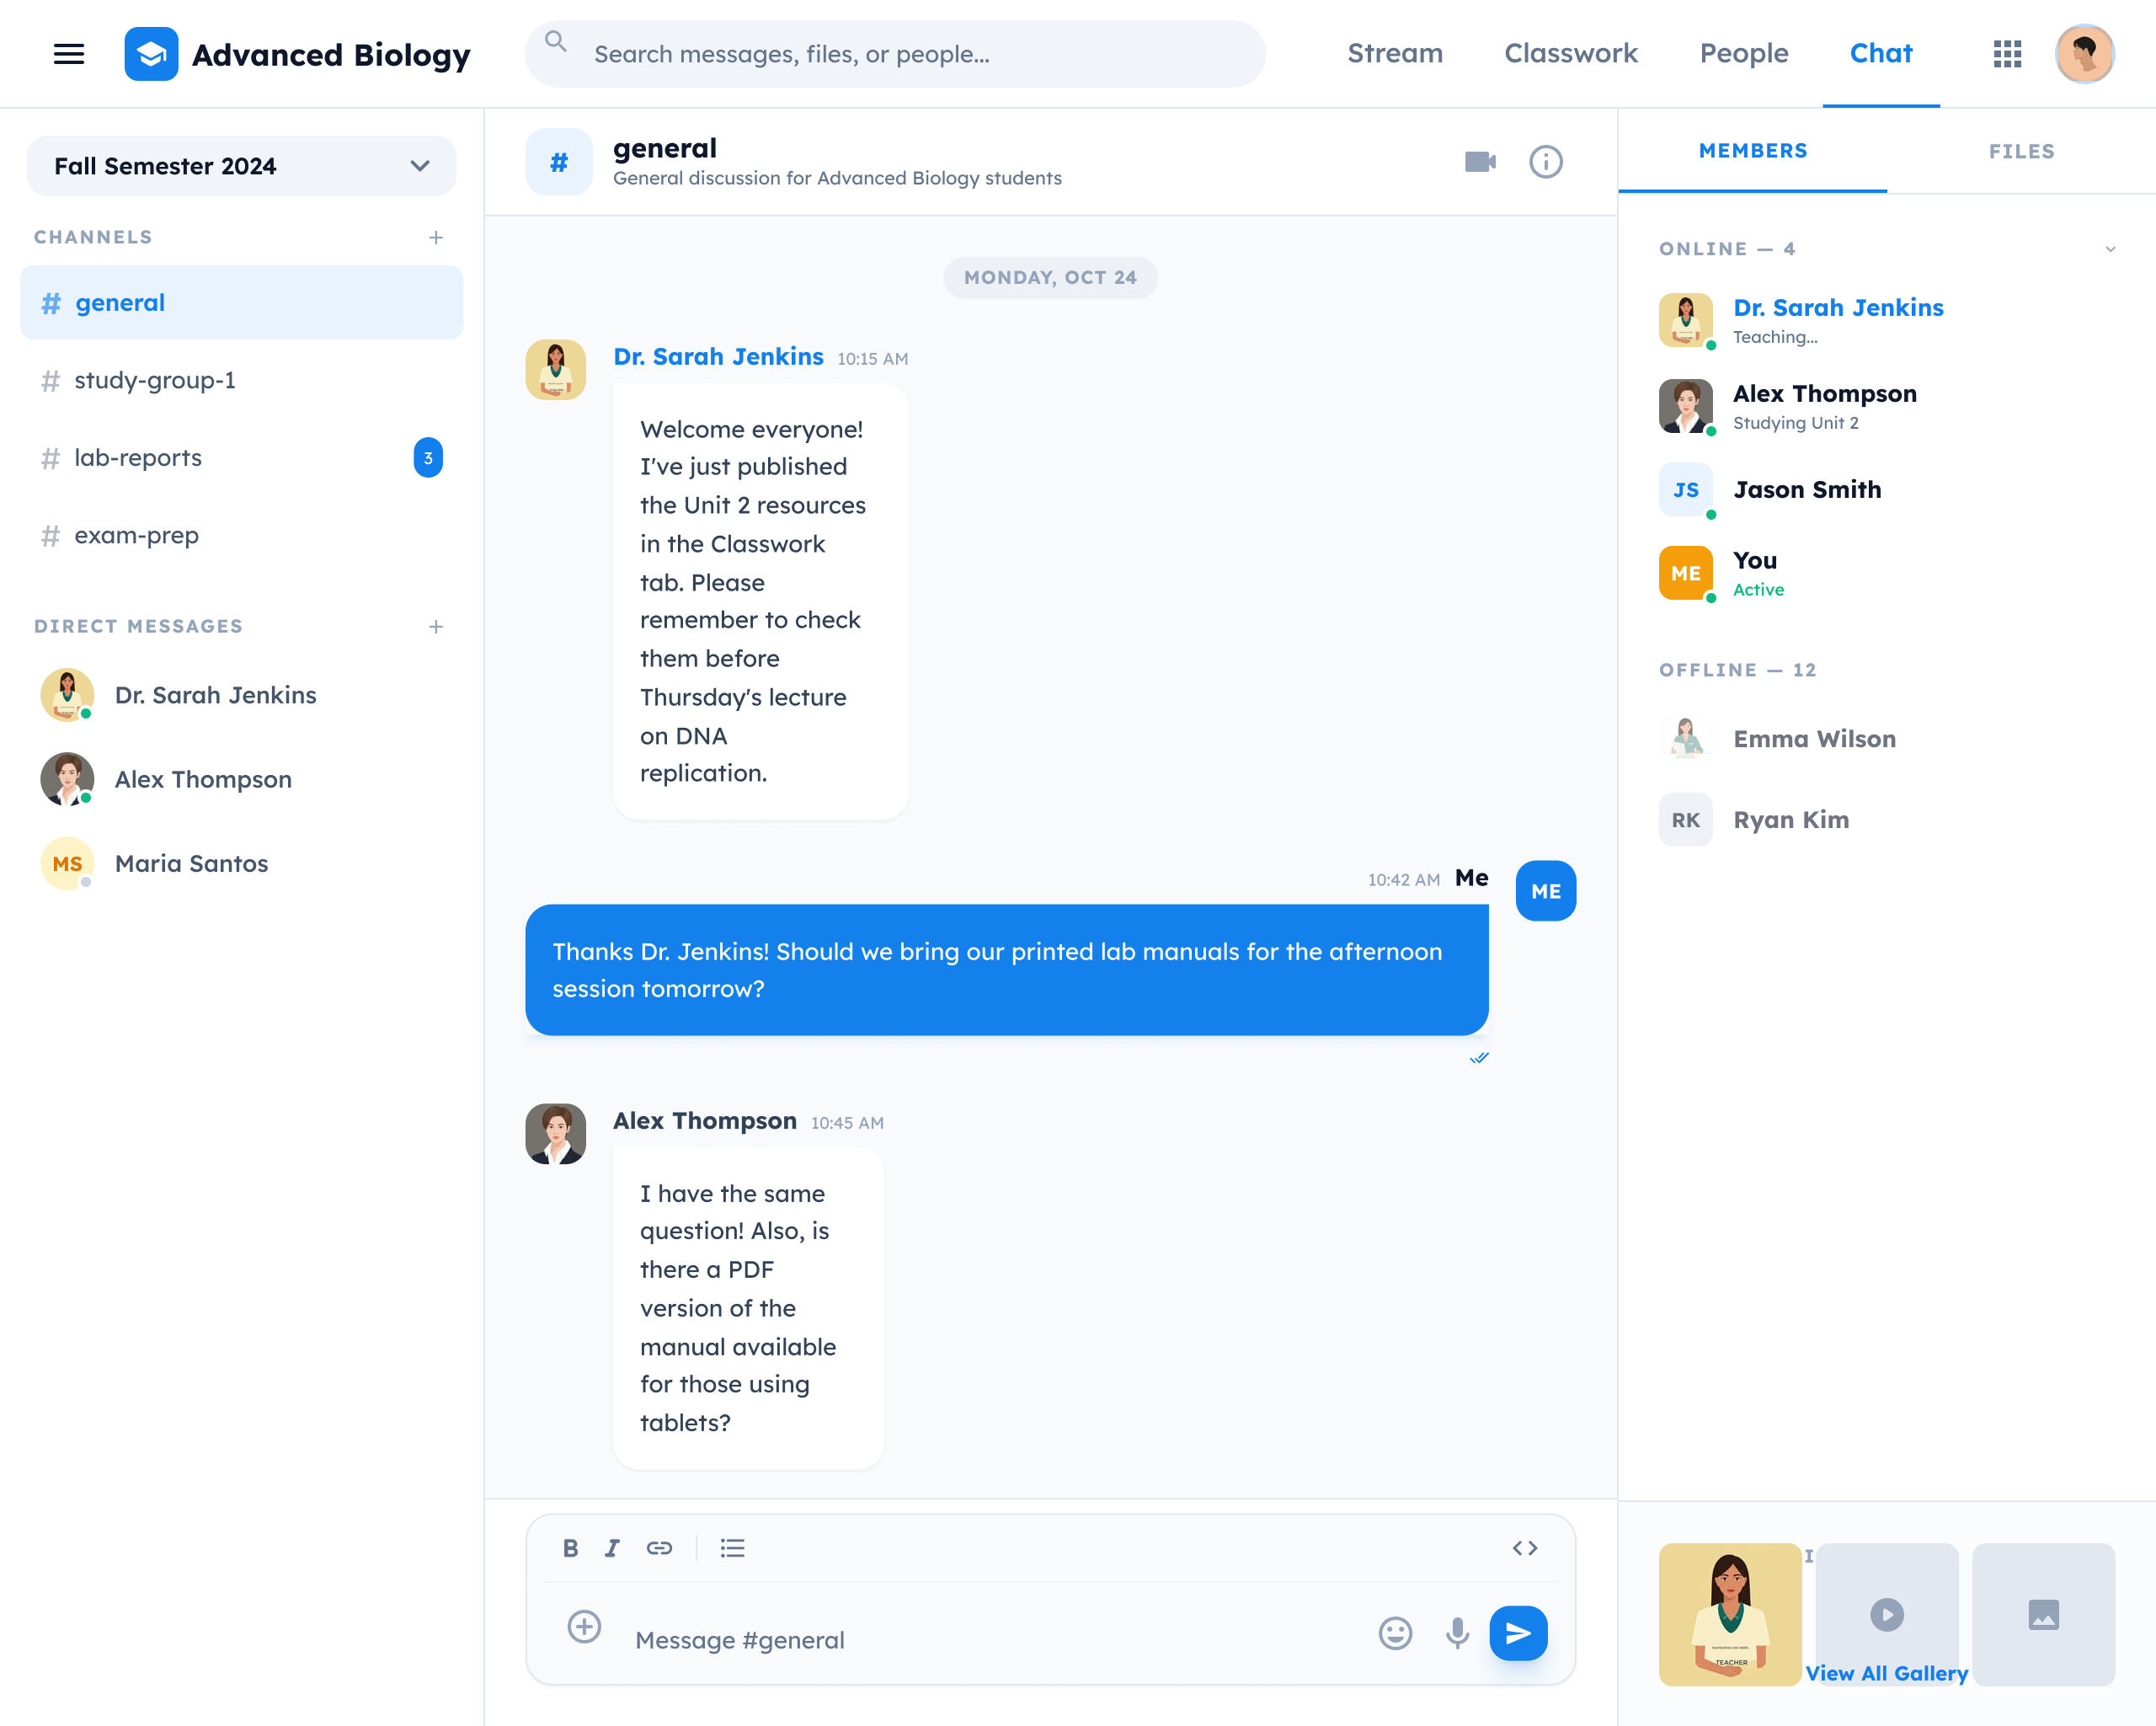
\includegraphics[width=0.85\textwidth]{figma/12 chat-page.png}
  \caption{Figma mockup of the real-time group chat interface.}
  \label{fig:figma-chat}
\end{figure}

% ── Notifications ───────────────────────────────────────────────────────────
\subsubsection{Notification System}

\begin{enumerate}[label=\textbf{FR-\arabic*.}, leftmargin=2.5cm, resume]
  \item \textbf{Event-driven notifications.}
        The system generates notifications for key events:
        \begin{itemize}[nosep]
          \item A new post is created in a classroom.
          \item An assignment is due within 24 hours.
          \item A submission has been graded.
          \item A new chat message is received (when the user is not active in the chat).
        \end{itemize}

  \item \textbf{Real-time delivery.}
        Notifications are pushed to connected clients in real time via Redis Pub/Sub.
        An unread count badge is displayed in the navigation bar.

  \item \textbf{Notification management.}
        Users can view their notifications, mark them as read (individually or all at once), and delete them (individually or all at once).
\end{enumerate}

\medskip

In total, 34 functional requirements were identified across various domains: authentication and user management, classroom management, member management, chapter management, post management, assignment and grading, file management, group chat, notifications, and search.

% ─────────────────────────────────────────────────────────────────────────────
\subsection{Non-Functional Requirements}
\label{sec:non-functional}

Beyond the functional capabilities, \eduspace{} must satisfy the following non-functional requirements to ensure a robust, secure, and maintainable system.

\begin{enumerate}[label=\textbf{NFR-\arabic*.}, leftmargin=2.8cm]
  \item \textbf{Performance.}
        \begin{itemize}[nosep]
          \item API response times must remain under 500\,ms for standard CRUD operations.
          \item Real-time chat messages must be delivered to all connected participants within 200\,ms under normal load.
          \item The search service must return results within 300\,ms for typical queries.
        \end{itemize}

  \item \textbf{Security.}
        \begin{itemize}[nosep]
          \item All passwords must be hashed using bcrypt before storage.
          \item Authentication is enforced via JWT tokens.
          \item WebSocket connections require a valid JWT token upon handshake.
        \end{itemize}

  \item \textbf{Scalability.}
        \begin{itemize}[nosep]
          \item The microservices architecture allows individual services to be scaled independently based on load.
          \item Each service owns its dedicated database.
        \end{itemize}

  \item \textbf{Availability and reliability.}
        \begin{itemize}[nosep]
          \item The system is containerized with Docker Compose, enabling reproducible deployments and rapid recovery.
          \item Service failures are isolated: if one microservice goes down, the rest continue to operate independently.
        \end{itemize}

  \item \textbf{Usability.}
        \begin{itemize}[nosep]
          \item The frontend provides a responsive, modern interface.
          \item Navigation is consistent across pages with a persistent sidebar and top navigation bar.
        \end{itemize}
\end{enumerate}

% =============================================================================
\section{Requirements Modeling}
\label{sec:modeling}

% ─────────────────────────────────────────────────────────────────────────────
\subsection{Use Case Diagrams}
\label{sec:use-case-diagrams}

\figref{fig:use-case-global} presents the global use case diagram of \eduspace{}, organized into seven functional packages: Authentication, Profile \& Account, Dashboard, Classroom Administration, Classroom Content, Assignments \& Grades, Chat, and Files.
The four actors---Visitor, User, Member, and Admin---interact with the system according to their privilege level.

\begin{figure}[H]
  \centering
  \rotatebox{90}{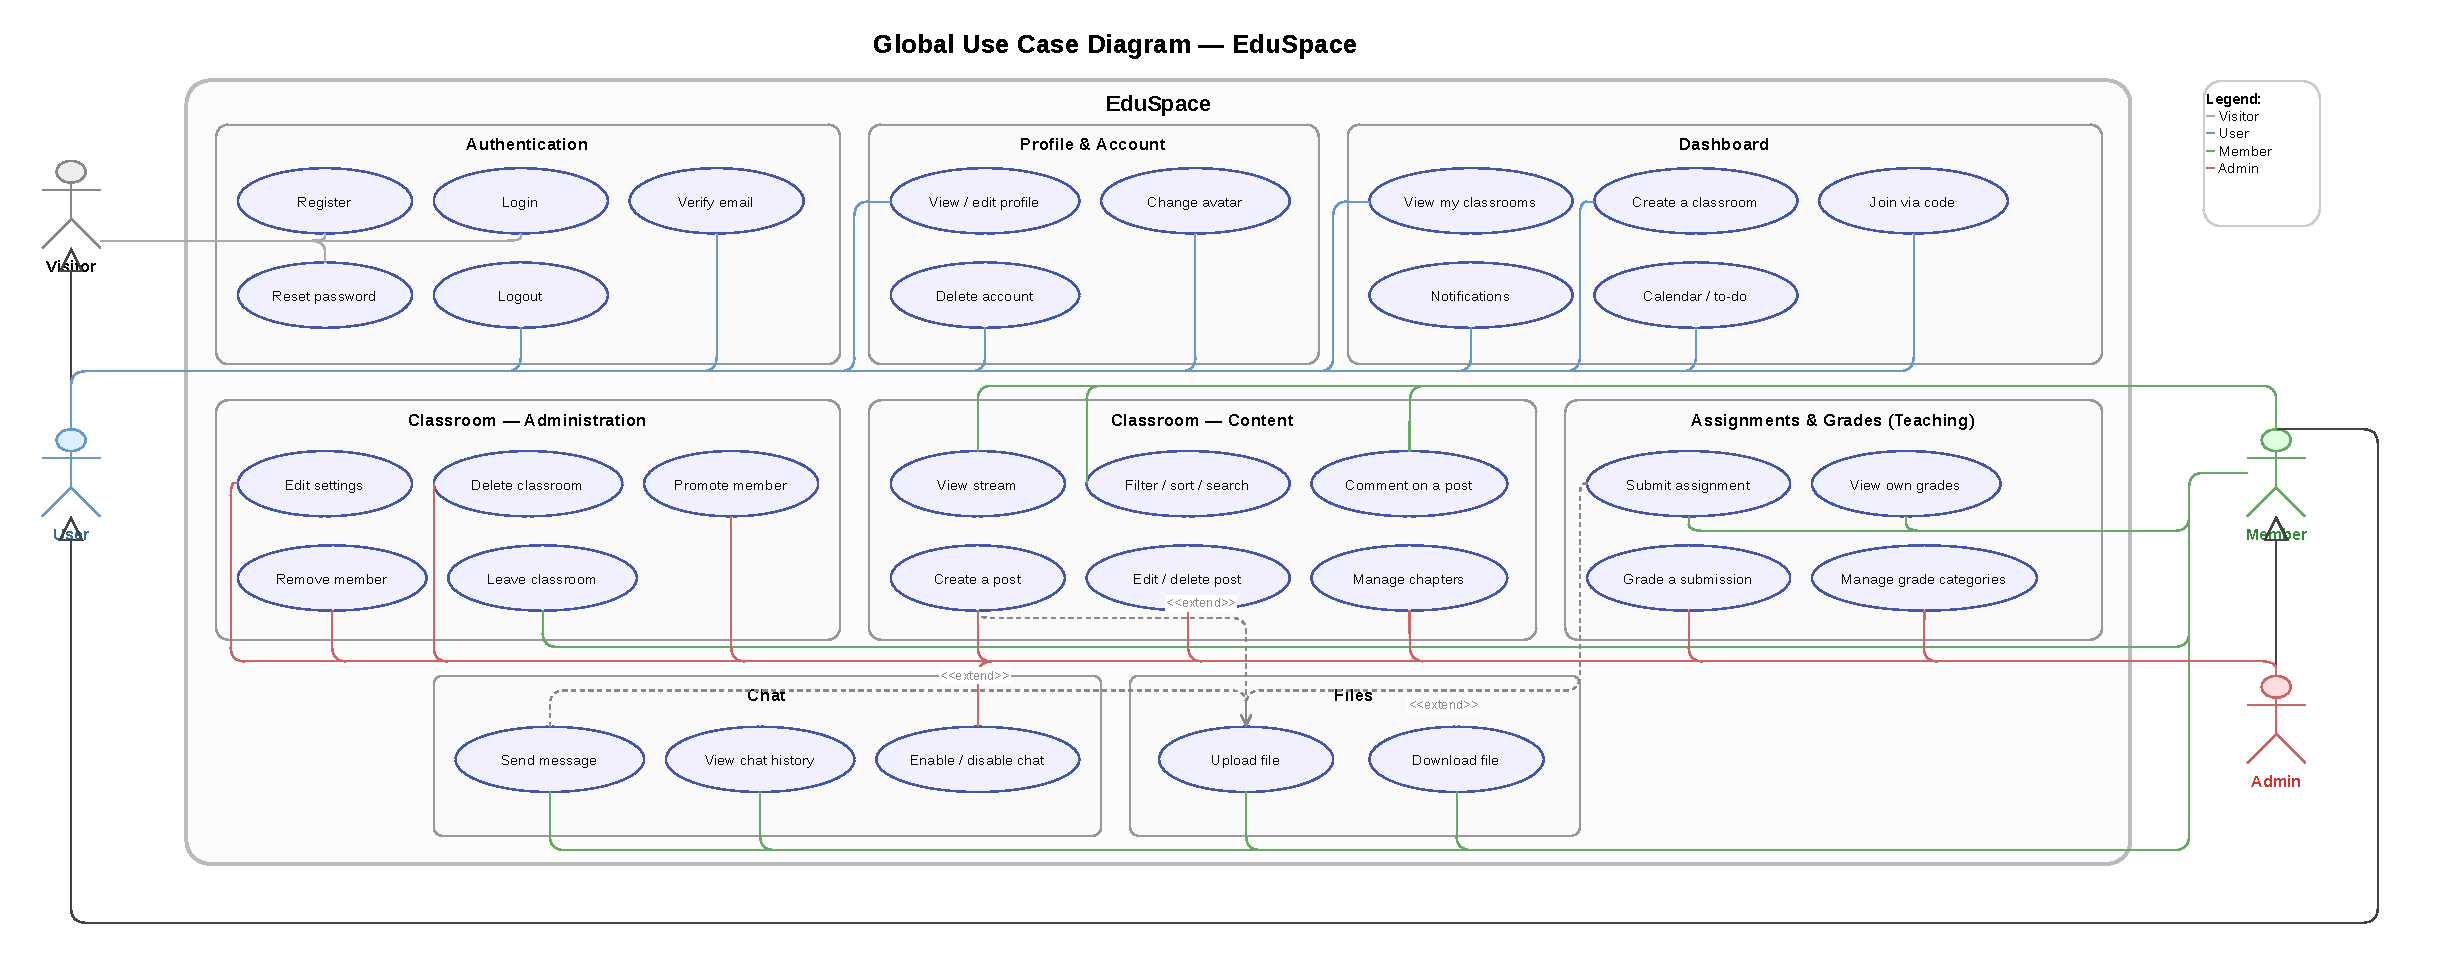
\includegraphics[width=0.85\textheight,height=\textwidth,keepaspectratio]{diagrams/use-case.pdf}}
  \caption{Global use case diagram of the \eduspace{} platform.}
  \label{fig:use-case-global}
\end{figure}

% ─────────────────────────────────────────────────────────────────────────────
\subsection{Use Case Descriptions}
\label{sec:use-case-descriptions}

This section describes the major use cases through nominal and alternative scenarios.

\subsubsection{UC-1: Register and Verify Email}

\begin{tabularx}{\textwidth}{@{} l X @{}}
  \toprule
  \textbf{Actor}          & Visitor \\
  \textbf{Precondition}   & The visitor has no existing account. \\
  \textbf{Postcondition}  & A verified user account exists; the user can log in. \\
  \midrule
  \multicolumn{2}{@{}l}{\textbf{Nominal scenario}} \\
  \midrule
  1 & The visitor opens the registration page. \\
  2 & The visitor fills in email, password, first name, and last name, then submits. \\
  3 & The system creates the account, hashes the password, generates a 6-digit code, and sends it by email. \\
  4 & The visitor enters the verification code. \\
  5 & The system marks the account as verified and redirects to the login page. \\
  \midrule
  \multicolumn{2}{@{}l}{\textbf{Alternative scenarios}} \\
  \midrule
  3a & Email already exists: the system returns an error. \\
  4a & Invalid code: the system displays an error; the user may request a new code. \\
  \bottomrule
\end{tabularx}

\subsubsection{UC-2: Login}

\begin{tabularx}{\textwidth}{@{} l X @{}}
  \toprule
  \textbf{Actor}          & Visitor \\
  \textbf{Precondition}   & The user has a verified account. \\
  \textbf{Postcondition}  & The user is authenticated and redirected to the dashboard. \\
  \midrule
  \multicolumn{2}{@{}l}{\textbf{Nominal scenario}} \\
  \midrule
  1 & The visitor opens the login page. \\
  2 & The visitor enters email and password, then submits. \\
  3 & The system validates credentials, generates a JWT token, and returns it with user profile data. \\
  4 & The frontend stores the token and redirects to the dashboard. \\
  \midrule
  \multicolumn{2}{@{}l}{\textbf{Alternative scenarios}} \\
  \midrule
  3a & Invalid credentials: the system returns a 401 error. \\
  3b & Email not verified: the system returns a 403 error and redirects to verification. \\
  \bottomrule
\end{tabularx}

\subsubsection{UC-3: Create a Classroom}

\begin{tabularx}{\textwidth}{@{} l X @{}}
  \toprule
  \textbf{Actor}          & User \\
  \textbf{Precondition}   & The user is authenticated. \\
  \textbf{Postcondition}  & A new classroom exists; the user is its creator (Admin). \\
  \midrule
  \multicolumn{2}{@{}l}{\textbf{Nominal scenario}} \\
  \midrule
  1 & The user clicks the create button on the dashboard. \\
  2 & The user fills in name, type (Teaching/Friendly), and optional fields (subject, section, description), then submits. \\
  3 & The system generates a unique 6-character class code, creates the classroom, adds the user as Admin, creates a ``General'' chapter, and publishes a \texttt{classroom.created} event. \\
  4 & The user is redirected to the new classroom. \\
  \bottomrule
\end{tabularx}

\subsubsection{UC-4: Create a Post}

\begin{tabularx}{\textwidth}{@{} l X @{}}
  \toprule
  \textbf{Actor}          & Admin \\
  \textbf{Precondition}   & The admin is in a classroom. \\
  \textbf{Postcondition}  & A new post appears in the stream; members are notified. \\
  \midrule
  \multicolumn{2}{@{}l}{\textbf{Nominal scenario}} \\
  \midrule
  1 & The admin opens the post creation form. \\
  2 & The admin selects a type, chapter, and fills in the title, content, and optional attachments. \\
  3 & If files are attached, they are uploaded to MinIO via the File Service. \\
  4 & The system verifies the admin's role, creates the post in a transaction, and publishes a \texttt{post.created} event. \\
  5 & The post appears in the stream; the Search Service indexes it; the Notification Service notifies members. \\
  \midrule
  \multicolumn{2}{@{}l}{\textbf{Alternative scenarios}} \\
  \midrule
  2a & Type is Assignment in a Friendly classroom: the API rejects the request with a 400 error. \\
  4a & User is not an Admin: the API returns a 403 error. \\
  \bottomrule
\end{tabularx}

\subsubsection{UC-5: Submit and Grade an Assignment}

\begin{tabularx}{\textwidth}{@{} l X @{}}
  \toprule
  \textbf{Actors}         & Member (submit), Admin (grade) \\
  \textbf{Precondition}   & An Assignment post exists in a Teaching classroom. \\
  \textbf{Postcondition}  & The submission is recorded and graded; the student is notified. \\
  \midrule
  \multicolumn{2}{@{}l}{\textbf{Nominal scenario}} \\
  \midrule
  1 & The member opens the assignment post and clicks submit. \\
  2 & The member optionally writes text and attaches files, then confirms. \\
  3 & The system uploads files, creates the submission, and displays a confirmation. \\
  4 & The admin views the list of submissions and selects one. \\
  5 & The admin enters points and optional feedback, then saves. \\
  6 & The system updates the submission, publishes \texttt{submission.graded}, and the student receives a notification. \\
  \midrule
  \multicolumn{2}{@{}l}{\textbf{Alternative scenarios}} \\
  \midrule
  5a & Points exceed the maximum: the API returns a 400 error. \\
  \bottomrule
\end{tabularx}

% ─────────────────────────────────────────────────────────────────────────────
\subsection{System Sequence Diagrams}
\label{sec:sequence-diagrams}

The following system sequence diagrams illustrate the interactions between the actors and the system for the major use cases.

\begin{figure}[H]
  \centering
  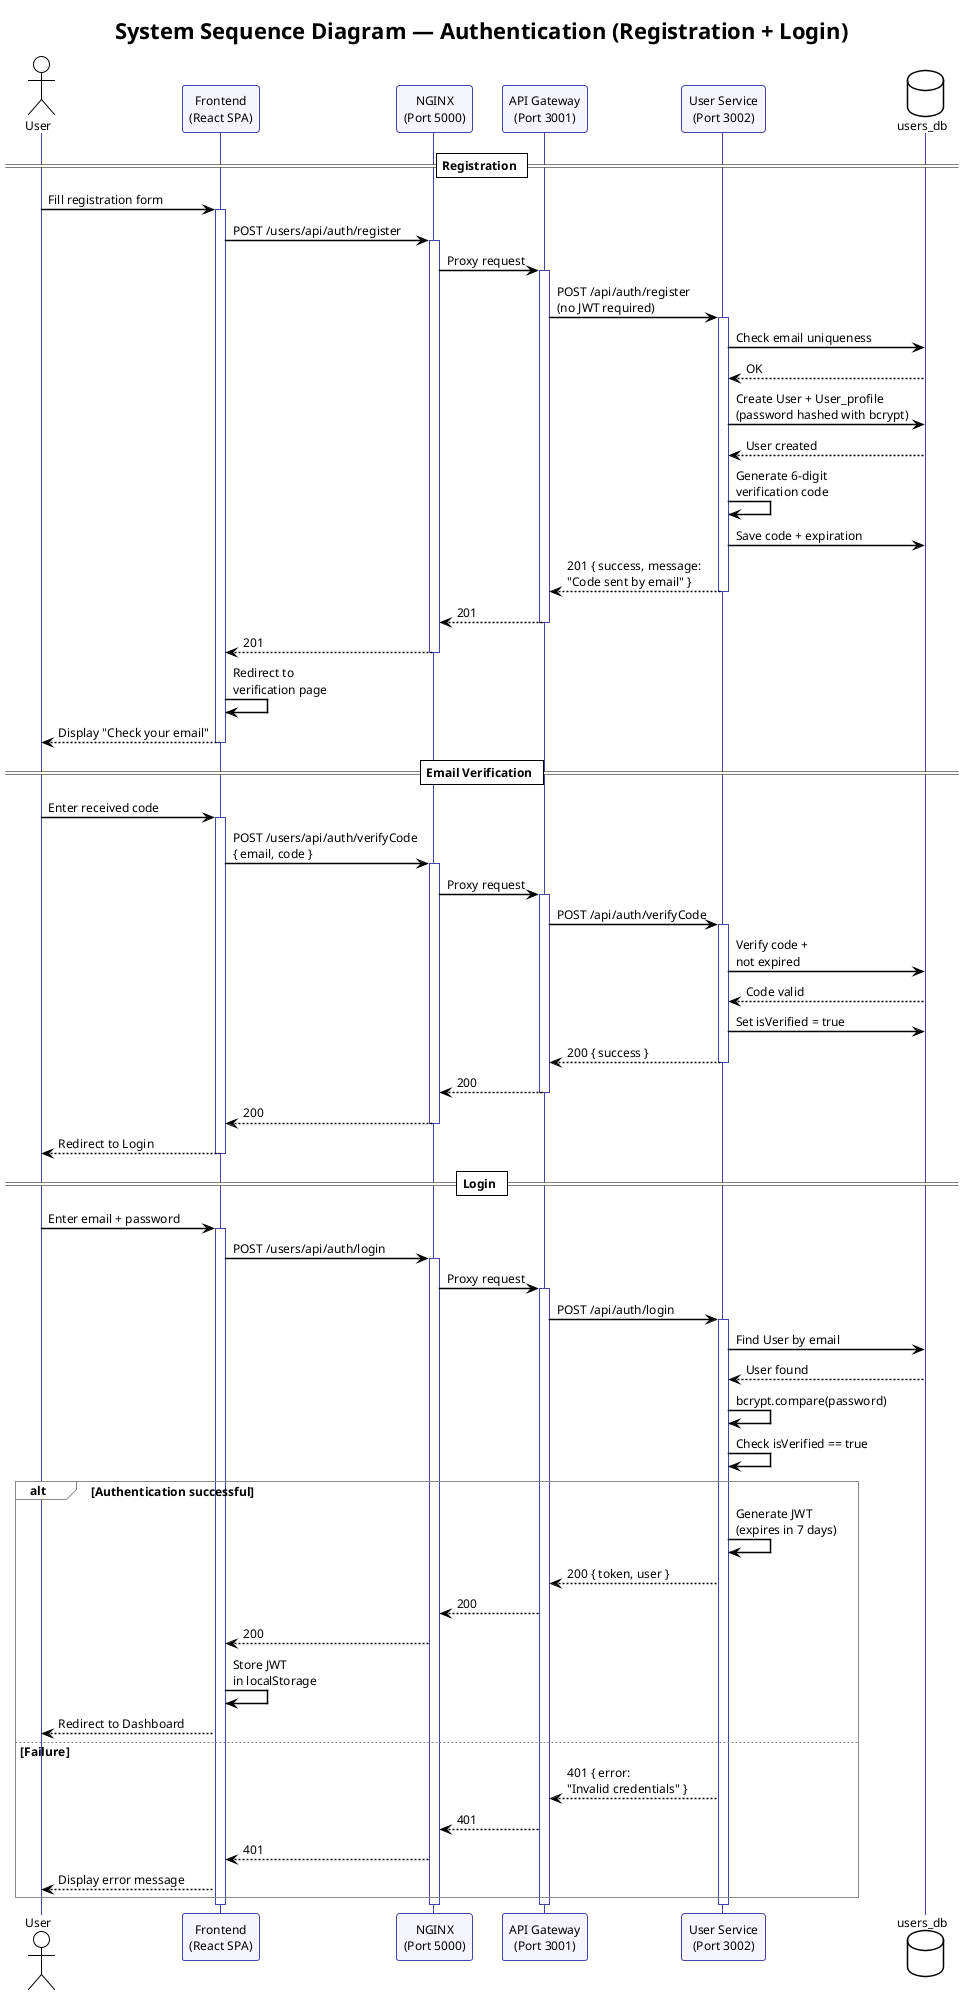
\includegraphics[width=\textwidth,height=0.85\textheight,keepaspectratio]{diagrams/seq-auth-login.png}
  \caption{System sequence diagram --- Authentication (Registration + Login).}
  \label{fig:seq-auth}
\end{figure}

\begin{figure}[H]
  \centering
  \rotatebox{90}{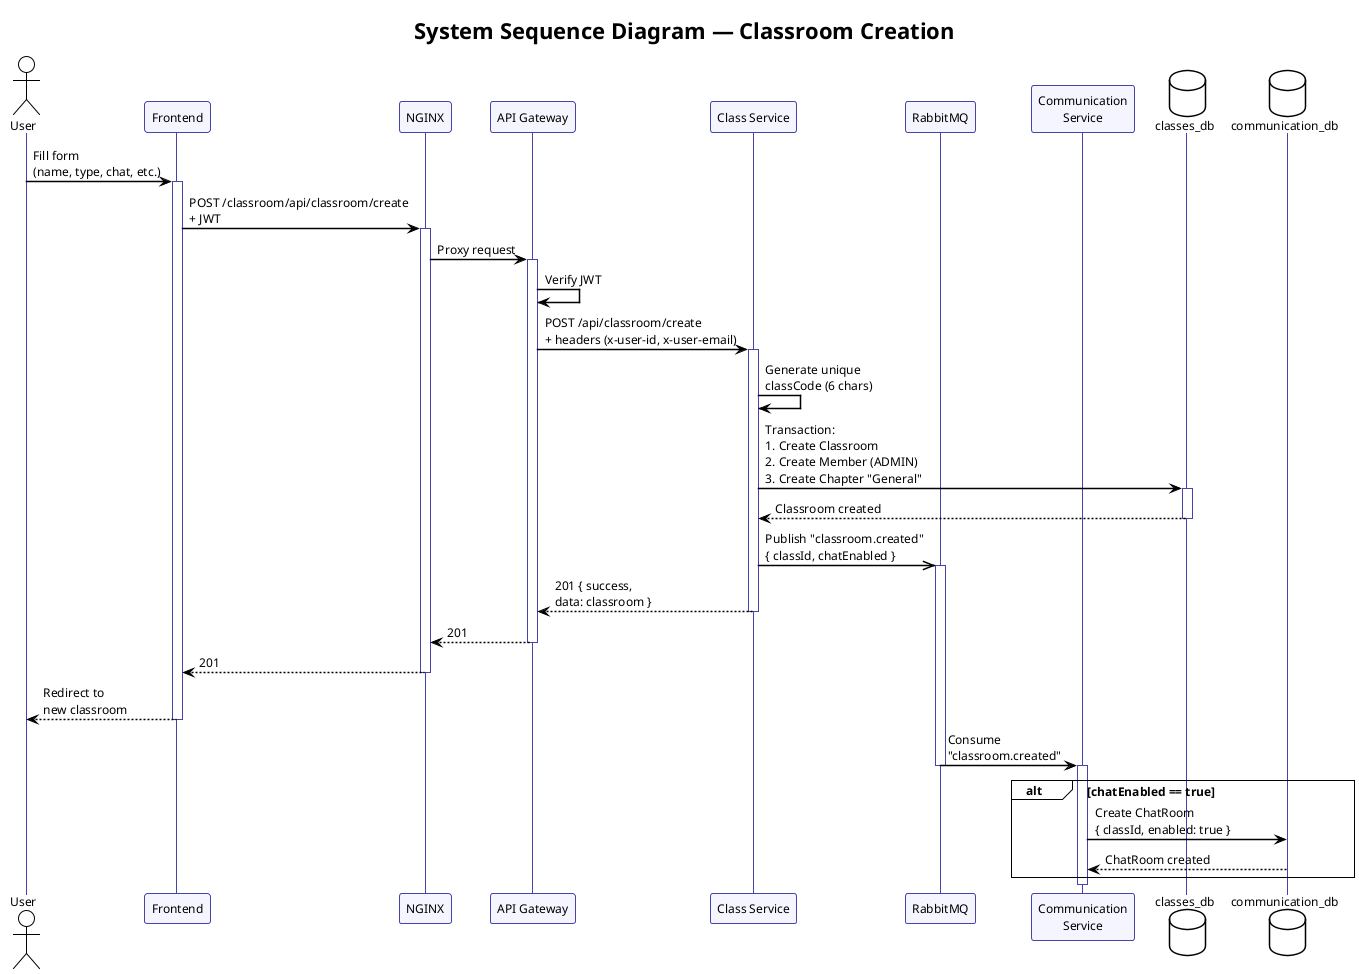
\includegraphics[width=0.85\textheight,height=\textwidth,keepaspectratio]{diagrams/seq-create-classroom.png}}
  \caption{System sequence diagram --- Classroom Creation.}
  \label{fig:seq-create-classroom}
\end{figure}

\begin{figure}[H]
  \centering
  \rotatebox{90}{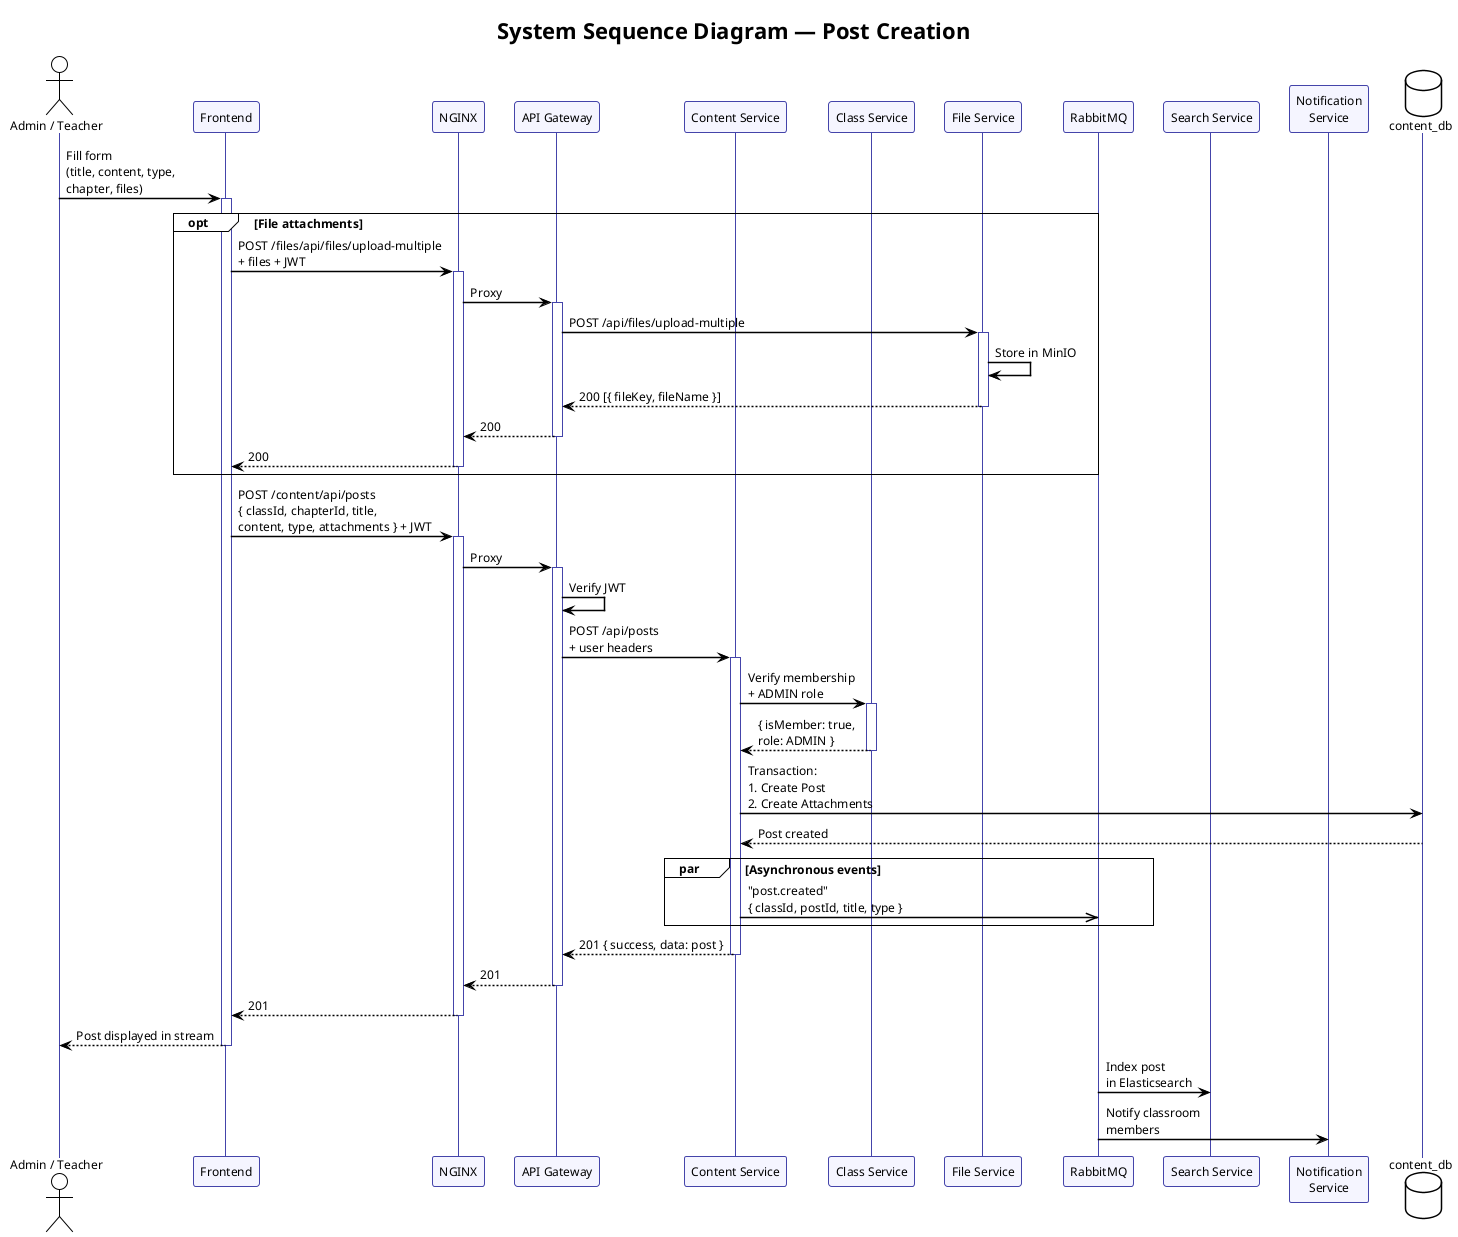
\includegraphics[width=0.85\textheight,height=\textwidth,keepaspectratio]{diagrams/seq-create-post.png}}
  \caption{System sequence diagram --- Post Creation.}
  \label{fig:seq-create-post}
\end{figure}

% Note: Section 2.2.4 "Contraintes techniques" is facultatif — omitted per instructions.

% ─────────────────────────────────────────────────────────────────────────────
\subsection{Task Distribution and Planning}
\label{sec:planning}

As described in \secref{sec:organization}, the team adopted a feature-based collaboration model.
Rather than dividing responsibilities along technical layers (frontend vs.\ backend), each team member took full ownership of specific features end-to-end---from database schema and backend API to the corresponding frontend interface.
Shared concerns such as UML diagrams, the shared utility package, infrastructure configuration, and architectural decisions were handled collaboratively.

The project was organized into six major phases, spanning approximately four months from February to May 2026.
\tabref{tab:phases} summarizes the phases and their scope.

\begin{table}[H]
  \centering
  \caption{Project phases and scope.}
  \label{tab:phases}
  \small
  \begin{tabularx}{\textwidth}{@{} c l X @{}}
    \toprule
    \textbf{Phase} & \textbf{Period} & \textbf{Scope} \\
    \midrule
    1 & Feb 1--14   & Requirements analysis, UML modeling, technology selection \\
    2 & Feb 15--28  & Infrastructure setup (Docker Compose, databases, Redis, RabbitMQ, MinIO, NGINX, Elasticsearch), shared package, API Gateway \\
    3 & Mar 1--Mar 15 & Core backend services: User, Class, Content, File \\
    4 & Mar 16--Mar 31   & Communication, Notification, and Search services; inter-service event wiring (RabbitMQ) \\
    5 & Apr 1--Apr 30 & Frontend development: authentication, dashboard, classroom pages, chat, grades, calendar, settings \\
    6 & May 1--May 19  & Integration testing, bug fixes, report writing \\
    \bottomrule
  \end{tabularx}
\end{table}


% =============================================================================
\section*{Conclusion}

This chapter defined the scope of \eduspace{} through a systematic requirements analysis.
A total of 34 functional requirements were identified across varoious domains, complemented by five non-functional requirements covering performance, security, scalability, availability, maintainability, and usability.
The UML modeling artifacts formalize the system's expected behavior and interactions.
The task distribution demonstrate how the two-person team organized the work across a five-month timeline.

The next chapter presents the system design, beginning with the architectural paradigm and proceeding to the object-oriented design artifacts.


% Chapter 3: System Design
% =============================================================================
% Chapter 3: System Design  (10–12 pages target)
% =============================================================================
\chapter{System Design}
\label{chap:design}

\section*{Introduction}

This chapter presents the architectural and object-oriented design of \eduspace{}.
It begins by justifying the choice of a microservices architectural paradigm and describing the overall system architecture, including the service decomposition, communication patterns, and infrastructure components.
The chapter then covers the object-oriented design artifacts: class diagrams, the persistence model, the attribute dictionary, and interaction modeling.

% =============================================================================
\section{General Architecture}
\label{sec:architecture}

% ─────────────────────────────────────────────────────────────────────────────
\subsection{Adopted Architectural Paradigm}
\label{sec:paradigm}

A fundamental design decision was whether to adopt a monolithic or a microservices architecture.
\tabref{tab:mono-vs-micro} summarizes the trade-offs between the two paradigms.

\begin{table}[H]
  \centering
  \caption{Comparison of monolithic and microservices architectures.}
  \label{tab:mono-vs-micro}
  \small
  \begin{tabularx}{\textwidth}{@{} l X X @{}}
    \toprule
    \textbf{Criterion} & \textbf{Monolithic} & \textbf{Microservices} \\
    \midrule
    Deployment        & Single unit; any change requires redeploying the entire application & Each service is deployed independently \\
    Database          & Single shared database; tight coupling between modules & Database-per-service; no shared state \\
    Scalability       & Entire application must be scaled uniformly & Individual services can be scaled based on load \\
    Fault isolation   & A failure in one module can bring down the entire system & Failures are contained within the affected service \\
    Complexity        & Lower operational complexity & Higher operational complexity (networking, orchestration) \\
    \bottomrule
  \end{tabularx}
\end{table}

The microservices approach was selected for \eduspace{} because the platform's functionality naturally decomposes into distinct bounded contexts (user management, classrooms, content, chat, notifications, search), each with its own data model and scaling characteristics~\cite{newman2021microservices}.
The database-per-service pattern~\cite{richardson2018microservices} prevents tight coupling, and different services have fundamentally different runtime needs---the communication service requires persistent WebSocket connections, the search service relies on Elasticsearch, and the file service is entirely stateless.

The backend is decomposed into seven domain services plus an API Gateway.
\tabref{tab:services} lists each service with its responsibility.

\begin{table}[H]
  \centering
  \caption{Service decomposition of the \eduspace{} backend.}
  \label{tab:services}
  \small
  \begin{tabularx}{\textwidth}{@{} l c c X @{}}
    \toprule
    \textbf{Service} & \textbf{Port} & \textbf{Database} & \textbf{Responsibility} \\
    \midrule
    API Gateway            & 3001 & ---               & JWT verification, rate limiting, request routing \\
    User Service           & 3002 & users\_db         & Authentication, profiles, password reset \\
    Class Service          & 3003 & classes\_db       & Classrooms, members, roles, chapters \\
    Content Service        & 3004 & content\_db       & Posts, comments, submissions, grading \\
    Communication Service  & 3005 & communication\_db & Real-time group chat, WebSocket, messages \\
    Notification Service   & 3006 & notifications\_db & Event-driven notifications, email delivery \\
    Search Service         & 3007 & --- (Elasticsearch) & Full-text search, post indexing \\
    File Service           & 3010 & --- (stateless)   & File upload/download via MinIO \\
    \bottomrule
  \end{tabularx}
\end{table}

Services communicate through two complementary patterns.
\textbf{Synchronous REST calls} are used when an immediate response is required---for example, the Content Service calls the Class Service to verify membership before any post operation.
\textbf{Asynchronous events via RabbitMQ} are used for fire-and-forget notifications: when a post is created, the Content Service publishes a \texttt{post.created} event consumed by the Notification and Search services, decoupling them temporally and preventing cascading failures.

All HTTP requests follow the path: React SPA $\rightarrow$ NGINX (port 5000) $\rightarrow$ API Gateway (JWT verification, rate limiting) $\rightarrow$ downstream service.
WebSocket connections for chat bypass the gateway and are proxied by NGINX directly to the Communication Service.
The infrastructure layer, orchestrated by Docker Compose, includes PostgreSQL (five databases), Redis, RabbitMQ, MinIO, Elasticsearch, and NGINX~\cite{postgresql2024docs,redis2024docs,rabbitmq2024docs,minio2024docs,elasticsearch2024docs,nginx2024docs}.

% ─────────────────────────────────────────────────────────────────────────────
\subsection{Functional Architecture (Site Map)}
\label{sec:sitemap}

\figref{fig:sitemap} presents the site map of \eduspace{}, showing the navigation structure between public pages (landing, login, registration, password reset) and protected pages (dashboard, calendar, to-do, settings, and classroom views).

\begin{figure}[H]
  \centering
  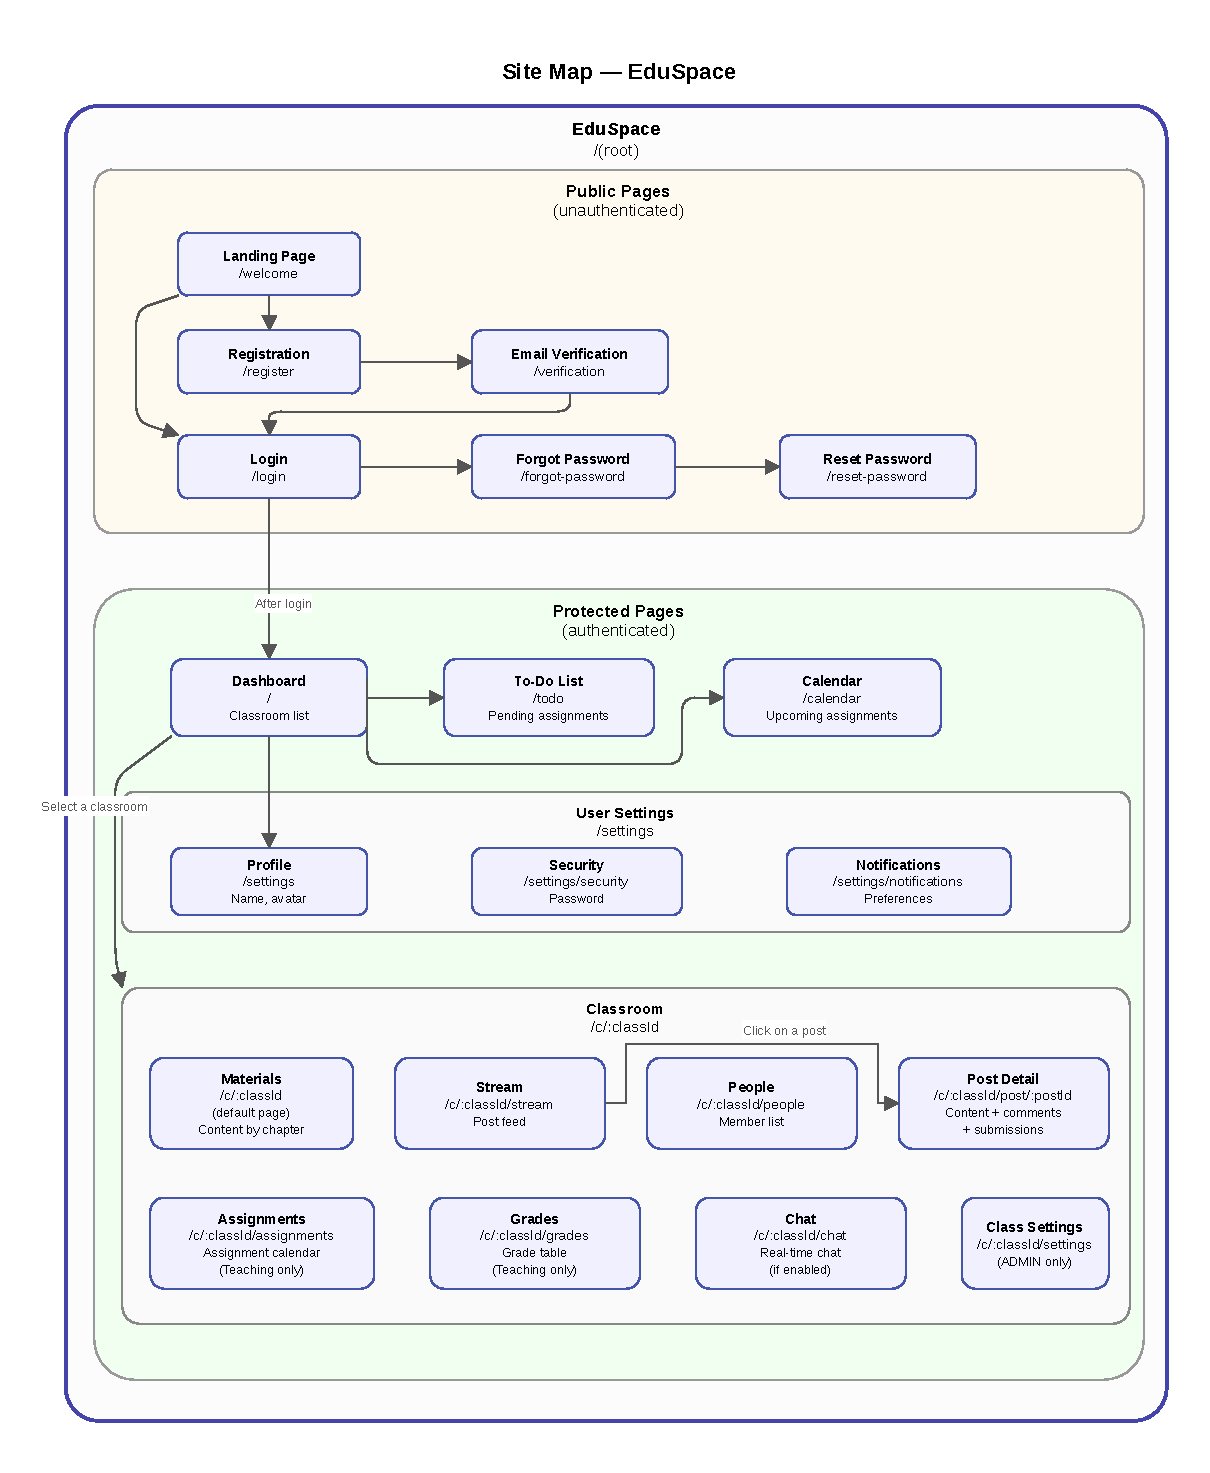
\includegraphics[width=\textwidth,height=0.85\textheight,keepaspectratio]{diagrams/sitemap.pdf}
  \caption{Site map of the \eduspace{} platform.}
  \label{fig:sitemap}
\end{figure}

% =============================================================================
\section{Object-Oriented Design}
\label{sec:oo-design}

% ─────────────────────────────────────────────────────────────────────────────
\subsection{Design Class Diagrams}
\label{sec:class-diagrams}

\figref{fig:class-design} presents the design class diagram, organized by service boundary.
Each service exposes controllers and data transfer objects (DTOs).
Inter-service dependencies are shown as REST calls (e.g., the Content Service calls the Class Service to verify membership).

\begin{figure}[H]
  \centering
  \rotatebox{90}{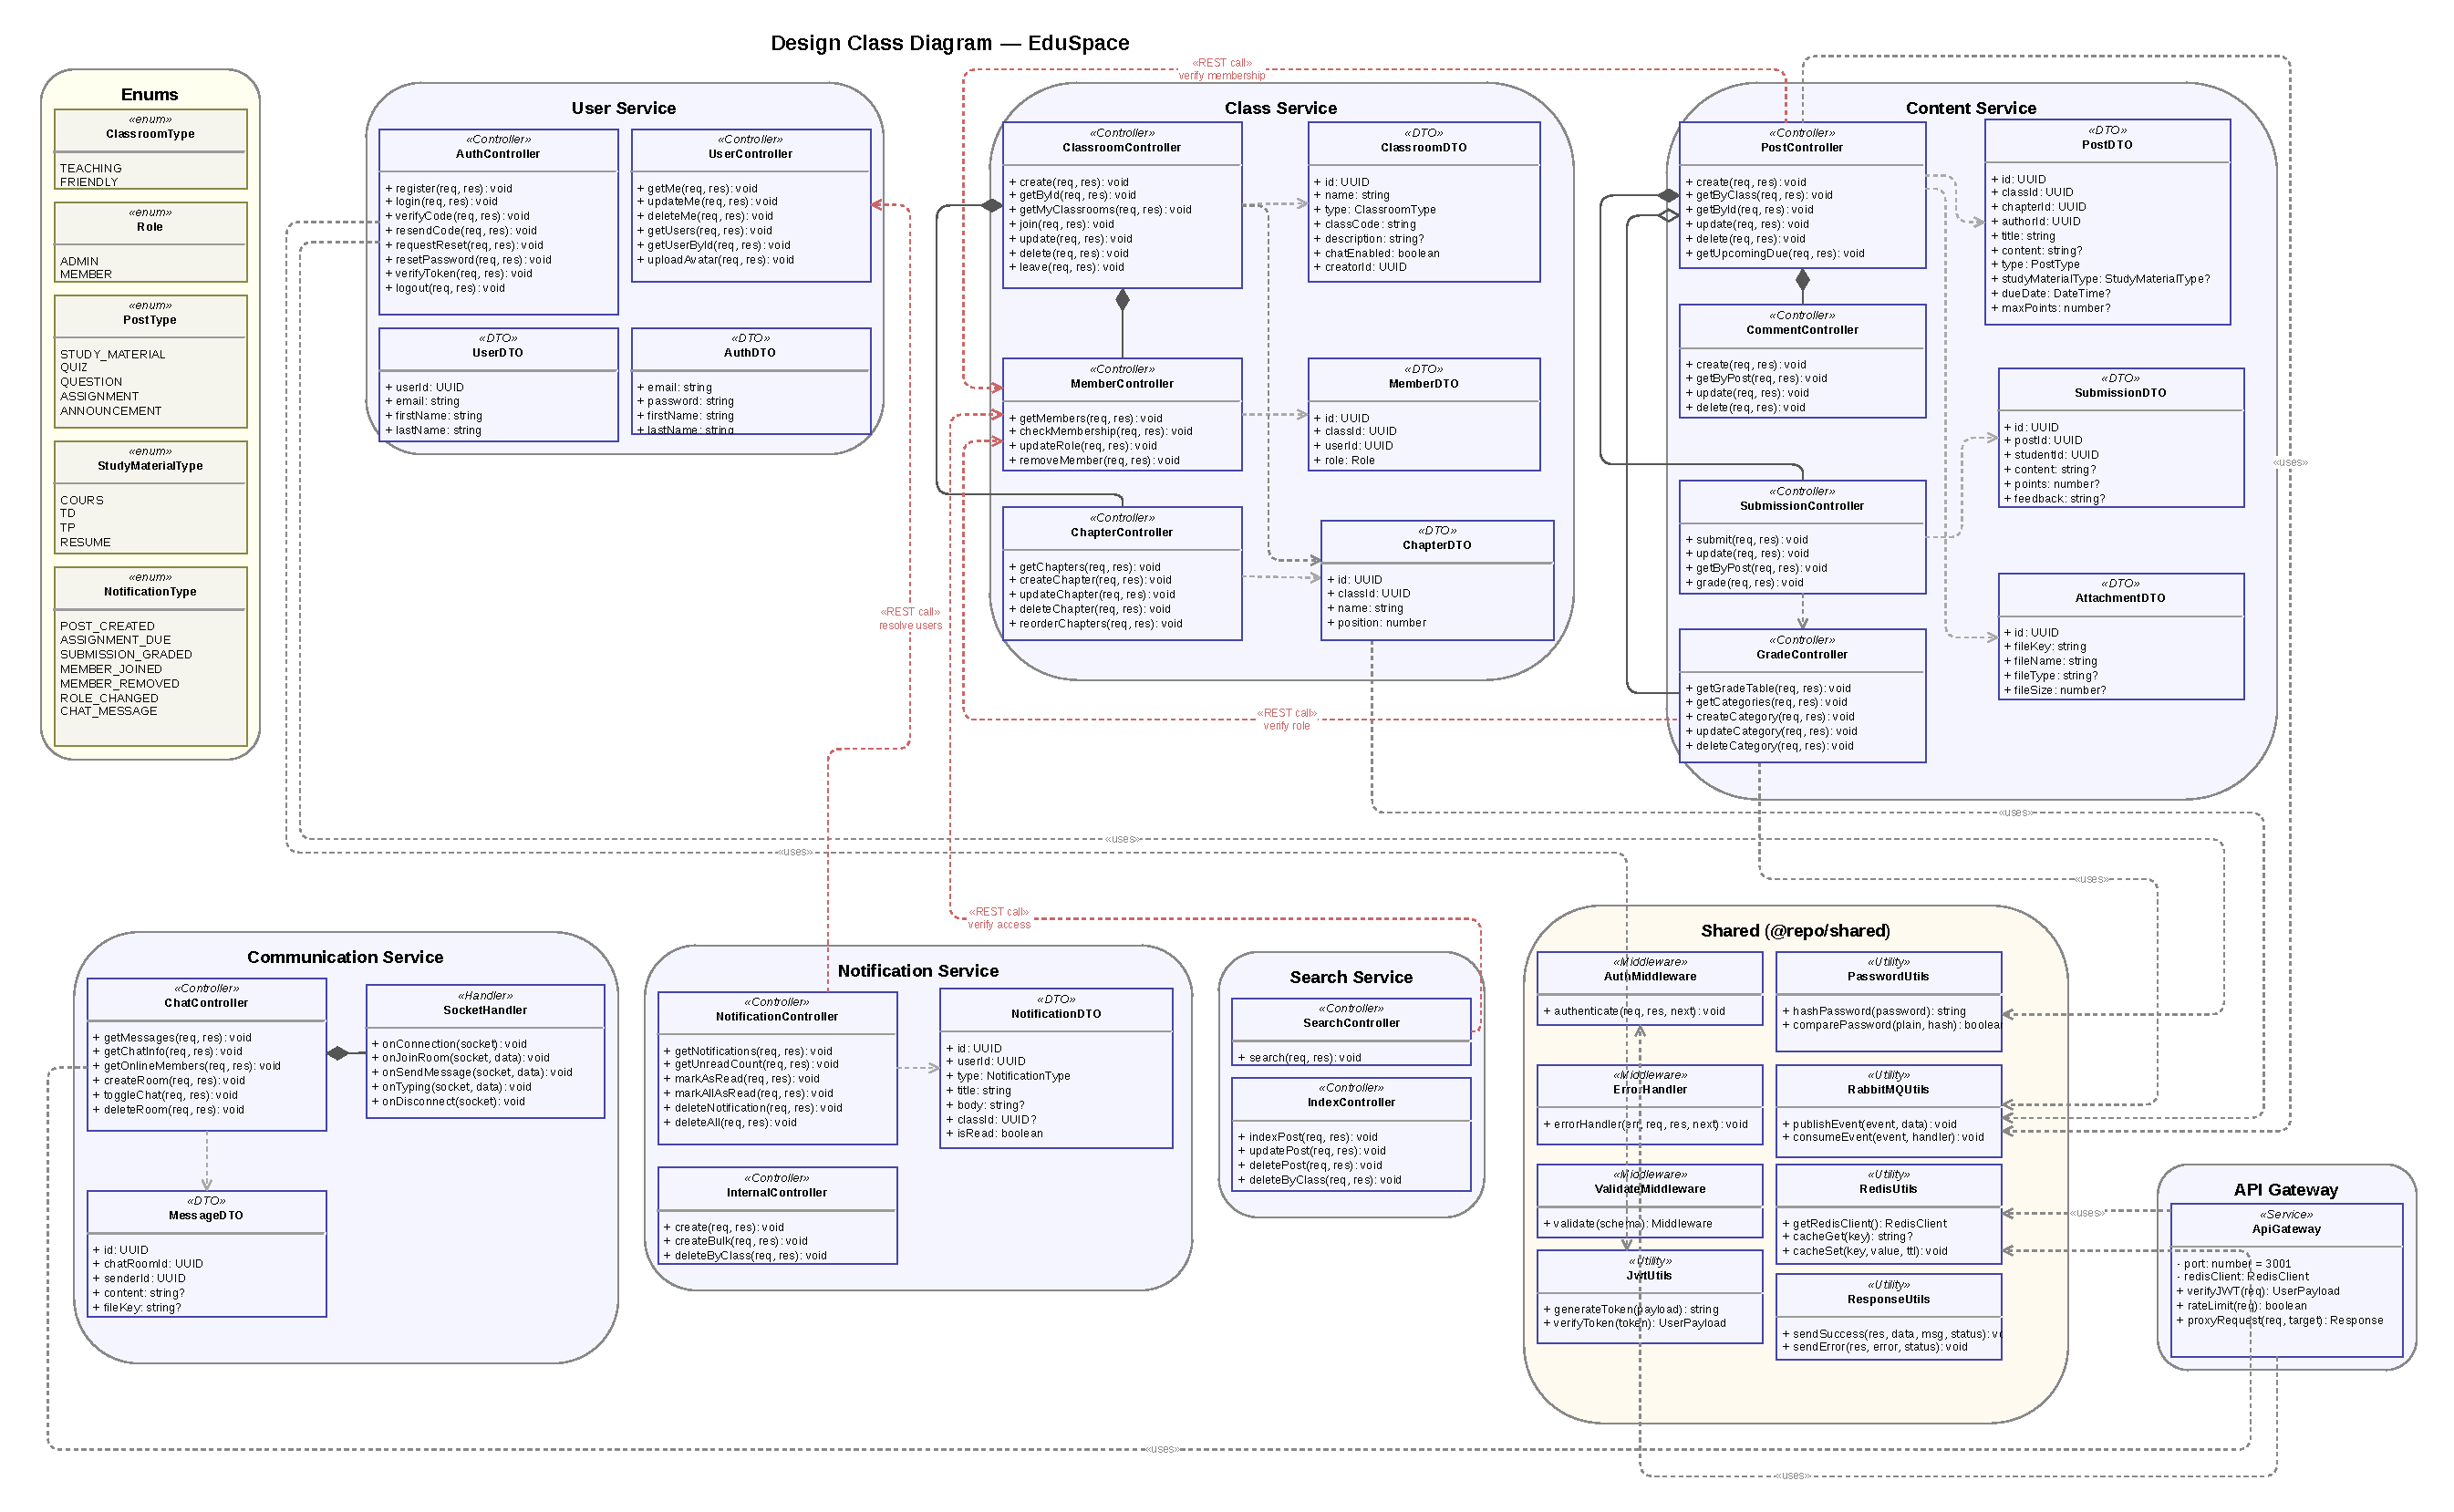
\includegraphics[width=0.85\textheight,height=\textwidth,keepaspectratio]{diagrams/class-design.pdf}}
  \caption{Design class diagram of \eduspace{}, organized by microservice.}
  \label{fig:class-design}
\end{figure}

% ─────────────────────────────────────────────────────────────────────────────
\subsection{Persistence Class Diagram}
\label{sec:persistence-diagram}

\figref{fig:class-persistence} presents the persistence class diagram, showing all entities across the five databases.
Each database boundary is color-coded: \texttt{users\_db}, \texttt{classes\_db}, \texttt{content\_db}, \texttt{communication\_db}, and \texttt{notifications\_db}.
Cross-database references (e.g., \texttt{class\_id} in the Content Service) are maintained as logical foreign keys, since each service owns its own database.

\begin{figure}[H]
  \centering
  \rotatebox{90}{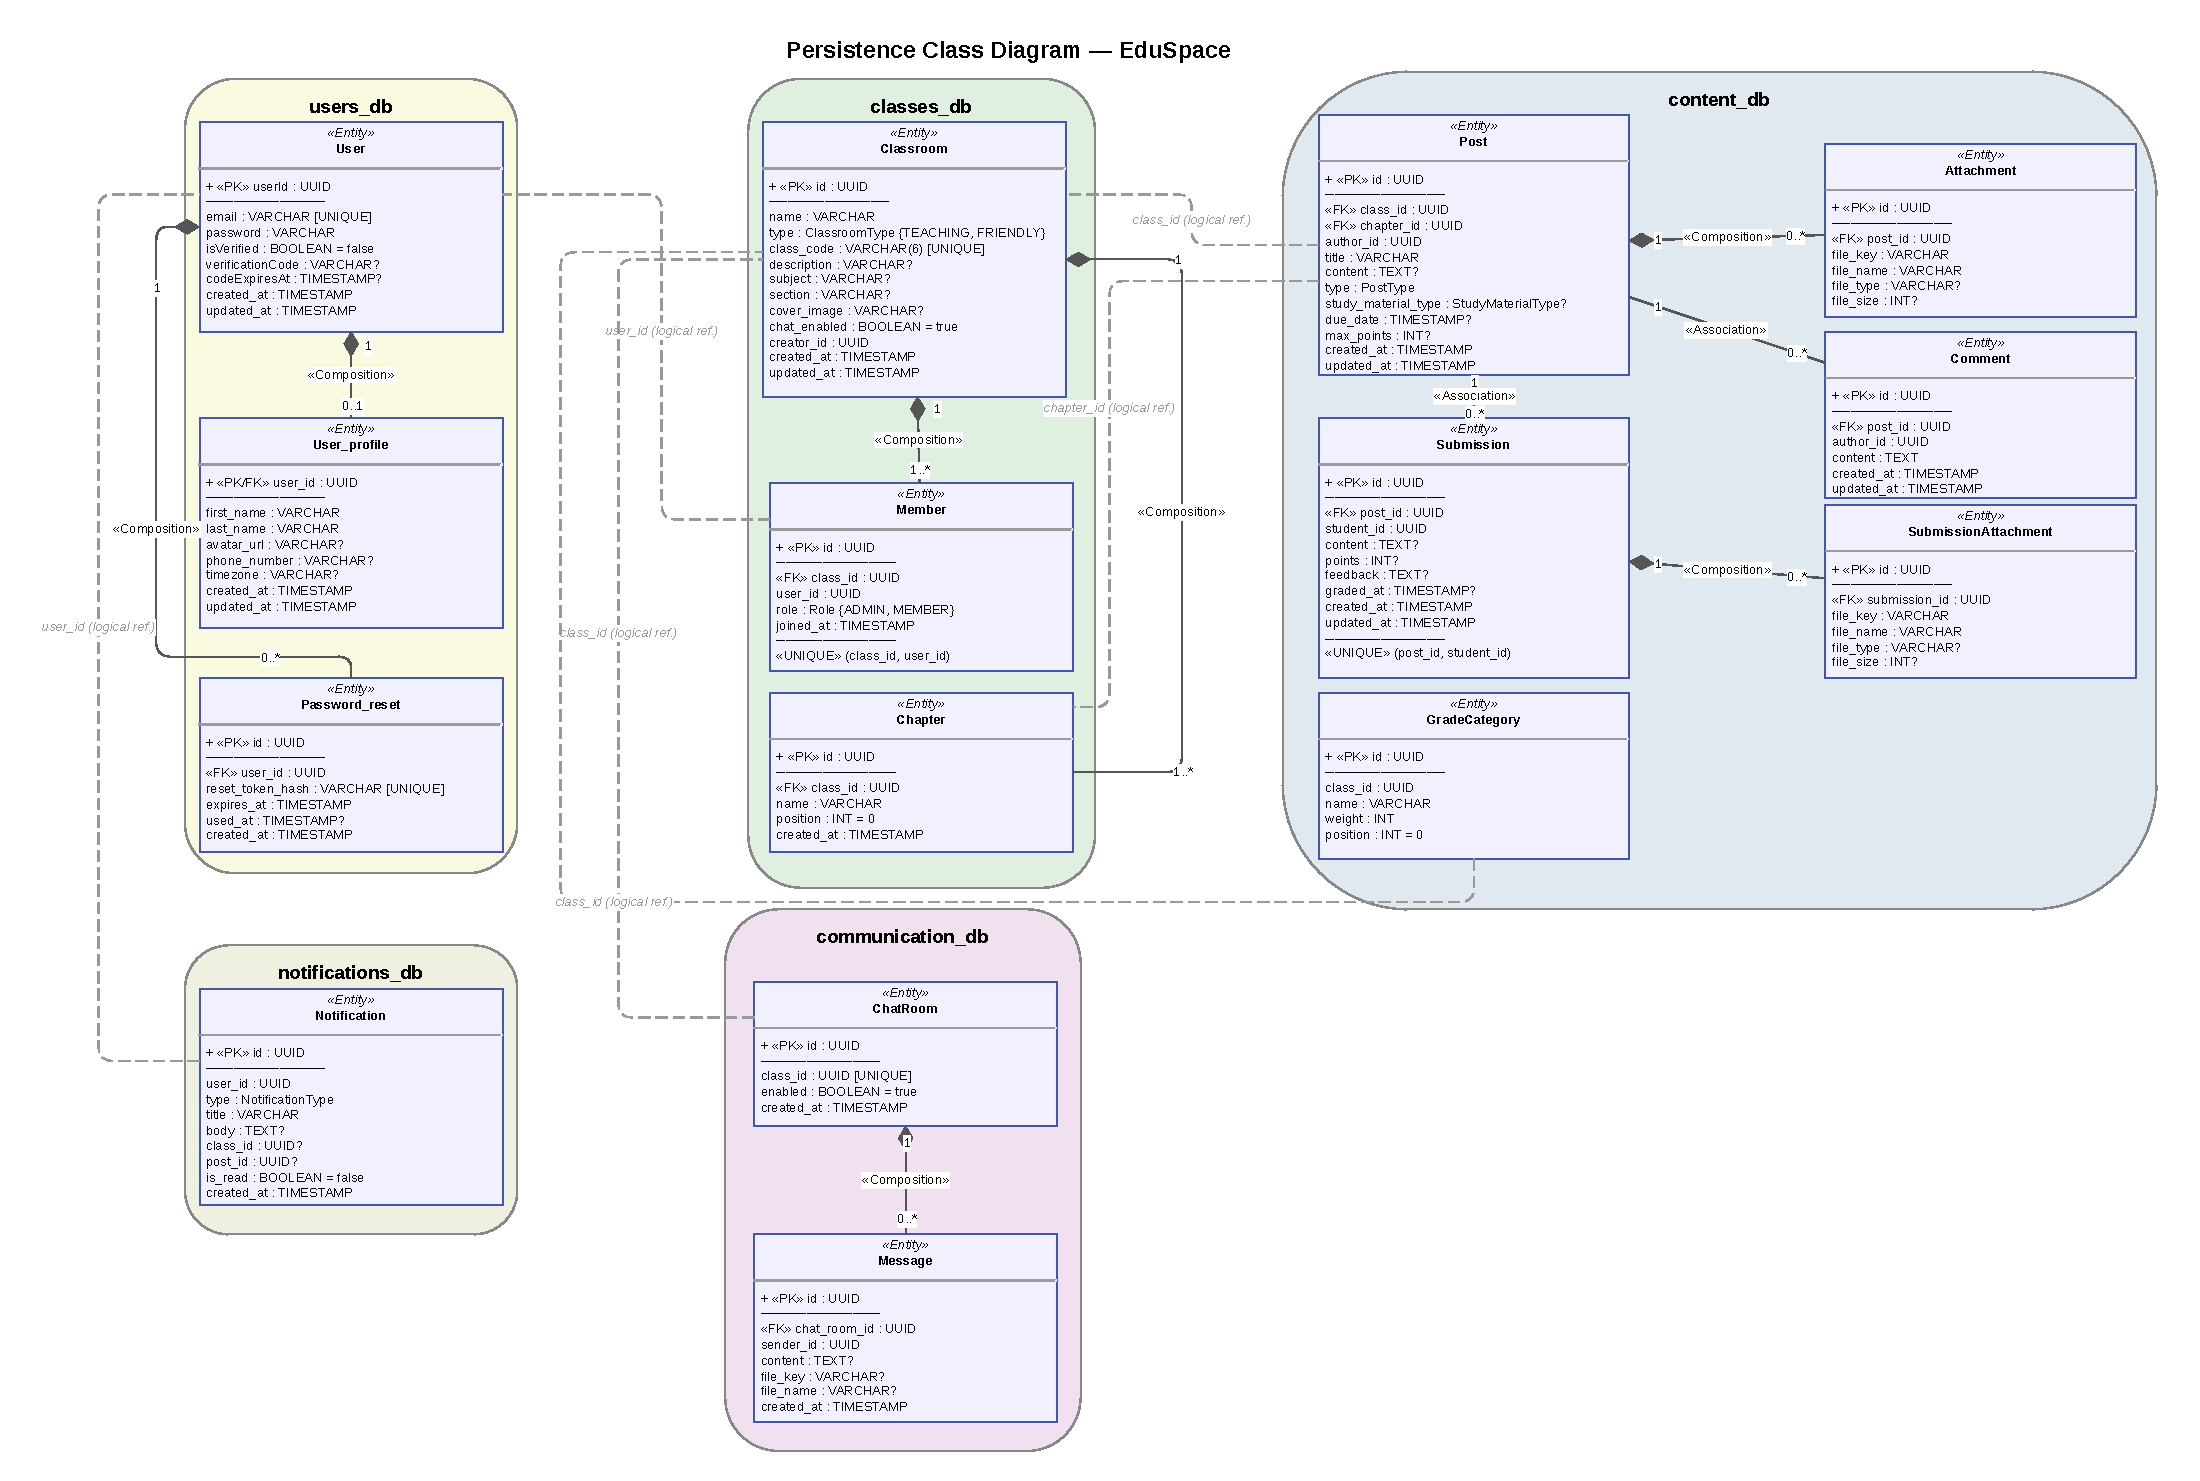
\includegraphics[width=0.85\textheight,height=\textwidth,keepaspectratio]{diagrams/class-persistence.pdf}}
  \caption{Persistence class diagram showing all entities across the five databases.}
  \label{fig:class-persistence}
\end{figure}

% ─────────────────────────────────────────────────────────────────────────────
\subsection{Attribute Dictionary}
\label{sec:attribute-dictionary}

The following tables describe the key attributes of each entity, derived from the Prisma schema definitions.

\begin{longtable}{@{} l l l p{5.5cm} @{}}
  \caption{Attribute dictionary --- \texttt{users\_db}.} \label{tab:dict-users} \\
  \toprule
  \textbf{Entity} & \textbf{Attribute} & \textbf{Type} & \textbf{Description} \\
  \midrule
  \endfirsthead
  \toprule
  \textbf{Entity} & \textbf{Attribute} & \textbf{Type} & \textbf{Description} \\
  \midrule
  \endhead
  User & userId & UUID (PK) & Unique identifier \\
       & email & VARCHAR (UNIQUE) & User email address \\
       & password & VARCHAR & Bcrypt-hashed password \\
       & isVerified & BOOLEAN & Email verification status \\
       & verificationCode & VARCHAR? & 6-digit email verification code \\
       & codeExpiresAt & TIMESTAMP? & Expiry of verification code \\
  \midrule
  User\_profile & user\_id & UUID (PK, FK) & References User \\
               & first\_name & VARCHAR & First name \\
               & last\_name & VARCHAR & Last name \\
               & avatar\_url & VARCHAR? & URL to avatar in MinIO \\
               & phone\_number & VARCHAR? & Optional phone number \\
               & timezone & VARCHAR? & User timezone preference \\
  \midrule
  Password\_reset & id & UUID (PK) & Unique identifier \\
                 & user\_id & UUID (FK) & References User \\
                 & reset\_token\_hash & VARCHAR (UNIQUE) & SHA-256 hash of reset token \\
                 & expires\_at & TIMESTAMP & Token expiry time \\
                 & used\_at & TIMESTAMP? & When the token was used \\
  \bottomrule
\end{longtable}

\begin{longtable}{@{} l l l p{5.5cm} @{}}
  \caption{Attribute dictionary --- \texttt{classes\_db}.} \label{tab:dict-classes} \\
  \toprule
  \textbf{Entity} & \textbf{Attribute} & \textbf{Type} & \textbf{Description} \\
  \midrule
  \endfirsthead
  \toprule
  \textbf{Entity} & \textbf{Attribute} & \textbf{Type} & \textbf{Description} \\
  \midrule
  \endhead
  Classroom & id & UUID (PK) & Unique identifier \\
            & name & VARCHAR & Classroom display name \\
            & type & ENUM & TEACHING or FRIENDLY \\
            & class\_code & VARCHAR(6) (UNIQUE) & 6-char join code \\
            & description & VARCHAR? & Optional description \\
            & subject & VARCHAR? & Subject or course name \\
            & section & VARCHAR? & Section/group label \\
            & cover\_image & VARCHAR? & Cover image file key \\
            & chat\_enabled & BOOLEAN & Whether chat is active \\
            & creator\_id & UUID & User who created the classroom \\
  \midrule
  Member & id & UUID (PK) & Unique identifier \\
         & class\_id & UUID (FK) & References Classroom \\
         & user\_id & UUID & References User (logical FK) \\
         & role & ENUM & ADMIN or MEMBER \\
         & joined\_at & TIMESTAMP & When the user joined \\
  \midrule
  Chapter & id & UUID (PK) & Unique identifier \\
          & class\_id & UUID (FK) & References Classroom \\
          & name & VARCHAR & Chapter title \\
          & position & INT & Display order (0-based) \\
  \bottomrule
\end{longtable}

\begin{longtable}{@{} l l l p{5.5cm} @{}}
  \caption{Attribute dictionary --- \texttt{content\_db}.} \label{tab:dict-content} \\
  \toprule
  \textbf{Entity} & \textbf{Attribute} & \textbf{Type} & \textbf{Description} \\
  \midrule
  \endfirsthead
  \toprule
  \textbf{Entity} & \textbf{Attribute} & \textbf{Type} & \textbf{Description} \\
  \midrule
  \endhead
  Post & id & UUID (PK) & Unique identifier \\
       & class\_id & UUID & Classroom (logical FK) \\
       & chapter\_id & UUID & Chapter (logical FK) \\
       & author\_id & UUID & Author (logical FK) \\
       & title & VARCHAR & Post title \\
       & content & TEXT? & Optional body text \\
       & type & ENUM & Post type (5 values) \\
       & study\_material\_type & ENUM? & Sub-type for STUDY\_MATERIAL \\
       & due\_date & TIMESTAMP? & Assignment due date \\
       & max\_points & INT? & Maximum grade points \\
  \midrule
  Attachment & id & UUID (PK) & Unique identifier \\
             & post\_id & UUID (FK) & References Post \\
             & file\_key & VARCHAR & MinIO object key \\
             & file\_name & VARCHAR & Original file name \\
             & file\_type & VARCHAR? & MIME type \\
             & file\_size & INT? & Size in bytes \\
  \midrule
  Submission & id & UUID (PK) & Unique identifier \\
             & post\_id & UUID (FK) & References Post (assignment) \\
             & student\_id & UUID & Student (logical FK) \\
             & content & TEXT? & Optional text content \\
             & points & INT? & Awarded grade \\
             & feedback & TEXT? & Instructor feedback \\
             & graded\_at & TIMESTAMP? & When graded \\
  \midrule
  GradeCategory & id & UUID (PK) & Unique identifier \\
                & class\_id & UUID & Classroom (logical FK) \\
                & name & VARCHAR & Category name \\
                & weight & INT & Weight percentage \\
                & position & INT & Display order \\
  \bottomrule
\end{longtable}

\begin{longtable}{@{} l l l p{5.5cm} @{}}
  \caption{Attribute dictionary --- \texttt{communication\_db} and \texttt{notifications\_db}.} \label{tab:dict-comm-notif} \\
  \toprule
  \textbf{Entity} & \textbf{Attribute} & \textbf{Type} & \textbf{Description} \\
  \midrule
  \endfirsthead
  \toprule
  \textbf{Entity} & \textbf{Attribute} & \textbf{Type} & \textbf{Description} \\
  \midrule
  \endhead
  ChatRoom & id & UUID (PK) & Unique identifier \\
           & class\_id & UUID (UNIQUE) & One chat room per classroom \\
           & enabled & BOOLEAN & Whether chat is active \\
  \midrule
  Message & id & UUID (PK) & Unique identifier \\
          & chat\_room\_id & UUID (FK) & References ChatRoom \\
          & sender\_id & UUID & Sender (logical FK) \\
          & content & TEXT? & Message text \\
          & file\_key & VARCHAR? & Attached file key \\
          & file\_name & VARCHAR? & Attached file name \\
  \midrule
  Notification & id & UUID (PK) & Unique identifier \\
               & user\_id & UUID & Target user (logical FK) \\
               & type & ENUM & Notification type (7 values) \\
               & title & VARCHAR & Notification title \\
               & body & TEXT? & Optional body text \\
               & class\_id & UUID? & Related classroom \\
               & post\_id & UUID? & Related post \\
               & is\_read & BOOLEAN & Read status \\
  \bottomrule
\end{longtable}

% ─────────────────────────────────────────────────────────────────────────────
\subsection{Interaction Modeling}
\label{sec:interaction-modeling}

The design-level sequence diagrams below detail the internal interactions within each service, showing routes, middleware, controllers, repositories, and utility classes.

\begin{figure}[H]
  \centering
  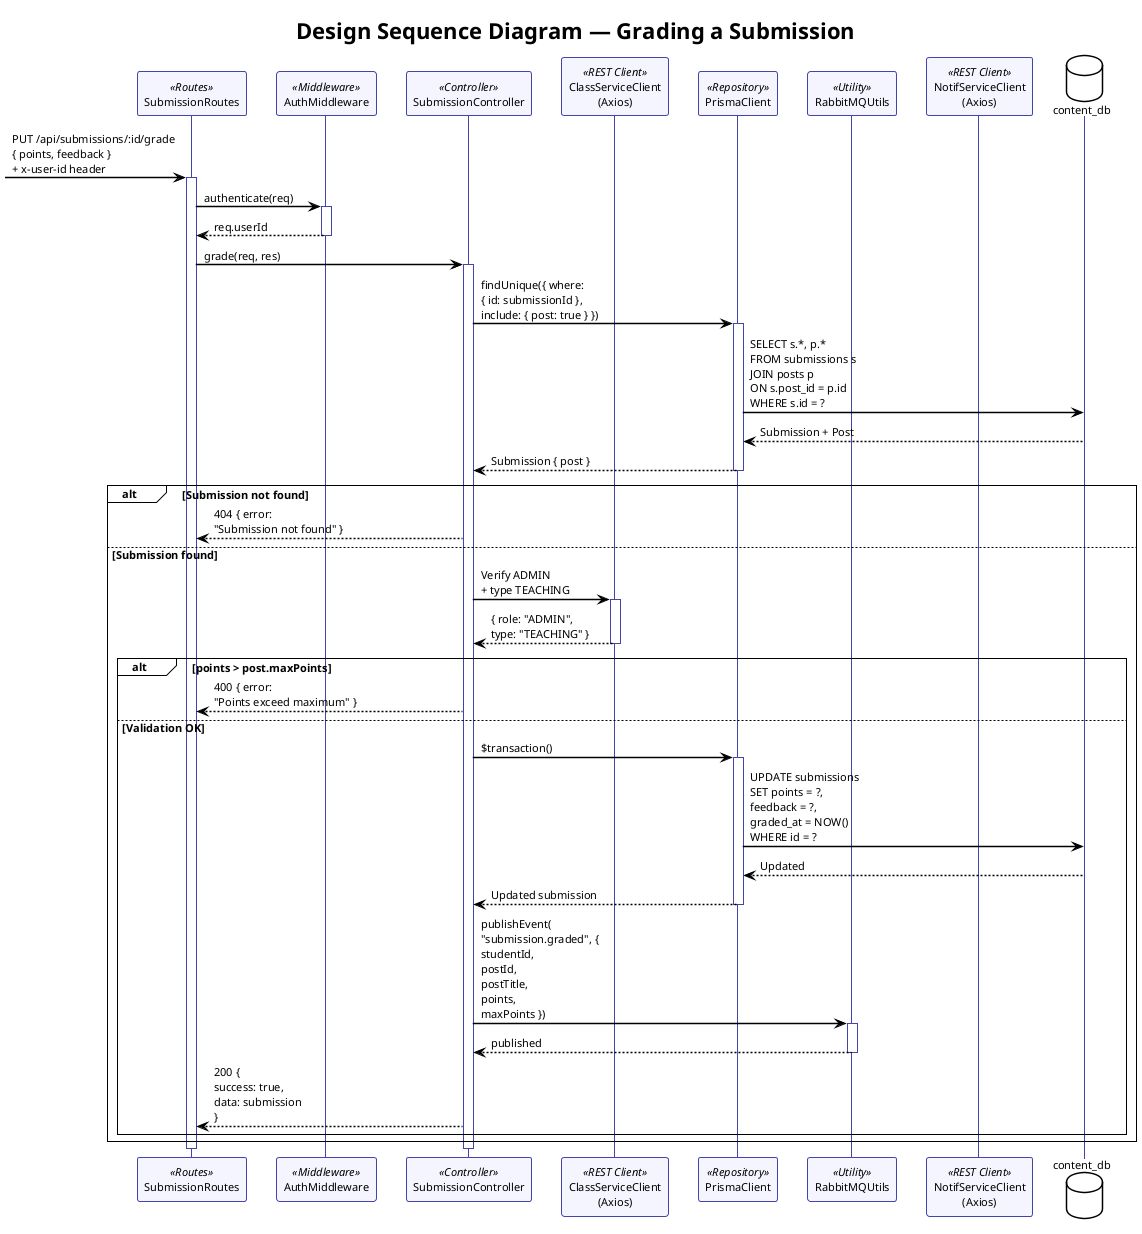
\includegraphics[width=\textwidth,height=0.85\textheight,keepaspectratio]{diagrams/seq-design-grade.png}
  \caption{Design sequence diagram --- Grading a Submission.}
  \label{fig:seq-design-grade}
\end{figure}

\begin{figure}[H]
  \centering
  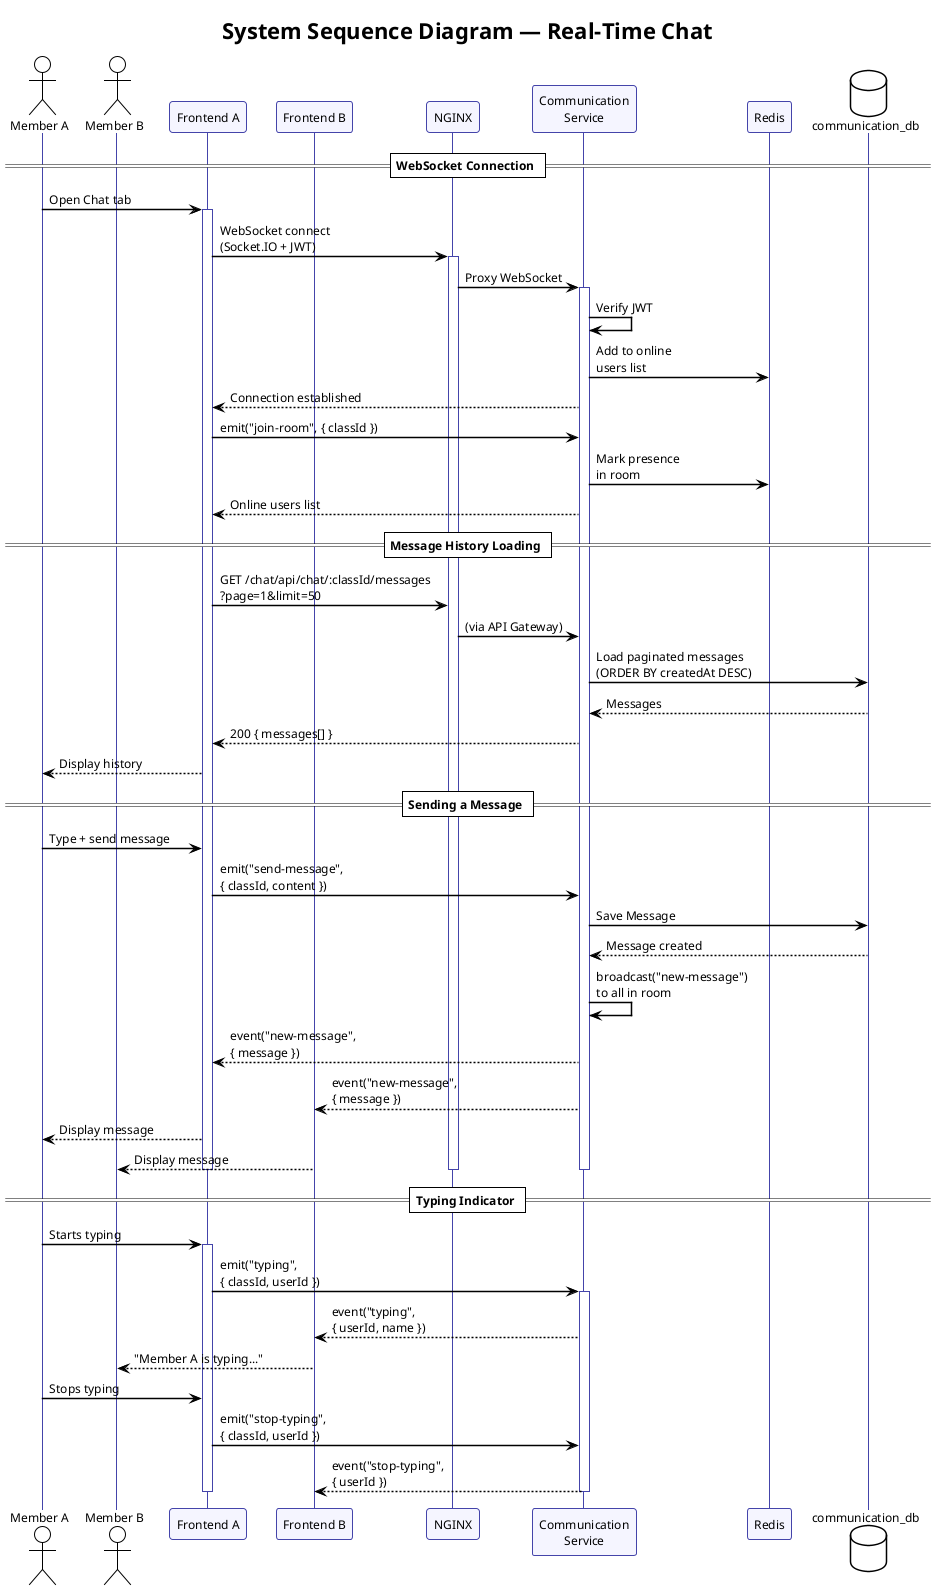
\includegraphics[width=\textwidth,height=0.85\textheight,keepaspectratio]{diagrams/seq-chat.png}
  \caption{System sequence diagram --- Real-Time Chat (WebSocket).}
  \label{fig:seq-chat}
\end{figure}

\begin{figure}[H]
  \centering
  \rotatebox{90}{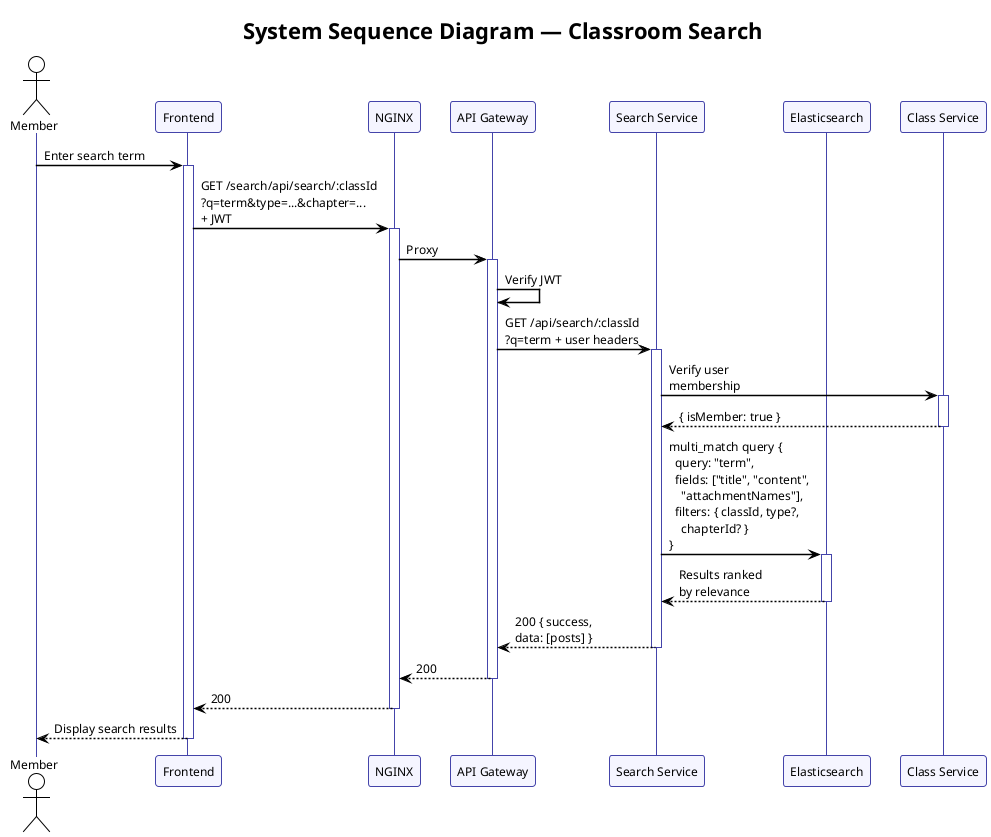
\includegraphics[width=0.85\textheight,height=\textwidth,keepaspectratio]{diagrams/seq-search.png}}
  \caption{System sequence diagram --- Classroom Search.}
  \label{fig:seq-search}
\end{figure}

% =============================================================================
\section*{Conclusion}

This chapter presented the system design of \eduspace{}.
The microservices architectural paradigm was justified based on domain alignment, independent data ownership, and technology suitability.
The overall architecture was described in detail, including the seven backend services, the API Gateway, the NGINX reverse proxy, the synchronous (REST) and asynchronous (RabbitMQ) communication patterns, and the infrastructure components managed by Docker Compose.
The object-oriented design artifacts---class diagrams, the persistence model, the attribute dictionary, and interaction diagrams---formalize the internal structure and dynamic behavior of the system.

The next chapter covers the implementation and deployment, detailing the technology stack, development environment, DevOps practices, security measures, and the user interfaces.


% Chapter 4: Implementation and Deployment
% =============================================================================
% Chapter 4: Implementation and Deployment  (14–18 pages target)
% =============================================================================
\chapter{Implementation and Deployment}
\label{chap:implementation}

\section*{Introduction}

This chapter details the concrete realization of the \eduspace{} platform.
It begins by describing the technological framework and development environment, covering both the hardware and software tools employed as well as the supporting configuration.
It then presents the DevOps and security practices adopted during development, including source code management, application security measures, and the design patterns leveraged throughout the codebase.
The chapter concludes with a presentation of the main user interfaces and their corresponding functionalities.

% =============================================================================
\section{Technological Framework and Development Environment}
\label{sec:tech-framework}

% ─────────────────────────────────────────────────────────────────────────────
\subsection{Hardware and Software Environment}
\label{sec:environment}

Development was carried out on personal machines running Linux (Ubuntu).
The following software tools and technologies were used across the project.

\subsubsection{Frontend Technologies}

\tabref{tab:frontend-stack} lists the frontend technology stack.

\begin{table}[H]
  \centering
  \caption{Frontend technology stack.}
  \label{tab:frontend-stack}
  \small
  \begin{tabularx}{\textwidth}{@{} l l X @{}}
    \toprule
    \textbf{Technology} & \textbf{Version} & \textbf{Purpose} \\
    \midrule
    React                & 19        & UI library for building the single-page application \\
    TypeScript           & 5         & Static type safety across the entire frontend codebase \\
    Vite                 & 6         & Build tool and development server with hot module replacement \\
    Tailwind CSS         & 4         & Utility-first CSS framework for responsive styling \\
    shadcn/ui + Radix UI & ---       & Accessible, composable component library \\
    React Router         & 7         & Client-side routing and navigation \\
    TanStack React Query & 5         & Server state management, caching, and data fetching \\
    TanStack React Table & 8         & Headless table library for the grades table \\
    FullCalendar         & 6         & Calendar component for assignment due date views \\
    Axios                & 1         & HTTP client for API communication \\
    Socket.IO Client     & 4         & WebSocket client for real-time group chat \\
    Lucide React         & ---       & Icon library \\
    \bottomrule
  \end{tabularx}
\end{table}

\subsubsection{Backend Technologies}

\tabref{tab:backend-stack} lists the backend technology stack, shared across all seven services and the API Gateway.

\begin{table}[H]
  \centering
  \caption{Backend technology stack.}
  \label{tab:backend-stack}
  \small
  \begin{tabularx}{\textwidth}{@{} l l X @{}}
    \toprule
    \textbf{Technology} & \textbf{Version} & \textbf{Purpose} \\
    \midrule
    Node.js          & 20 LTS    & JavaScript runtime for all backend services \\
    Express          & 5         & HTTP framework for REST API routing and middleware \\
    TypeScript       & 5         & Static type safety across all backend services \\
    Prisma ORM       & 6         & Type-safe database access, schema declaration, and migrations \\
    jsonwebtoken     & 9         & JWT creation and verification for authentication \\
    Multer           & 2         & Middleware for handling multipart file uploads \\
    Nodemailer       & 6         & Email sending for password reset and notification emails \\
    Morgan           & 1         & HTTP request logging middleware \\
    Socket.IO        & 4         & WebSocket server for real-time chat (Communication Service) \\
    amqplib          & 0.10      & RabbitMQ client for publishing and consuming events \\
    ioredis          & 5         & Redis client for caching, rate limiting, and Pub/Sub \\
    \bottomrule
  \end{tabularx}
\end{table}

\subsubsection{Infrastructure Technologies}

\tabref{tab:infra-stack} lists the infrastructure components, all orchestrated via Docker Compose.

\begin{table}[H]
  \centering
  \caption{Infrastructure technology stack.}
  \label{tab:infra-stack}
  \small
  \begin{tabularx}{\textwidth}{@{} l l X @{}}
    \toprule
    \textbf{Technology} & \textbf{Version} & \textbf{Purpose} \\
    \midrule
    PostgreSQL      & 16       & Relational database (five isolated databases) \\
    Redis           & 7        & Caching, rate limiting, presence tracking, Pub/Sub \\
    RabbitMQ        & 3.13     & Message broker for asynchronous inter-service events \\
    MinIO           & latest   & S3-compatible object storage for all binary files \\
    Elasticsearch   & 8        & Full-text search engine for post indexing and querying \\
    NGINX           & 1.25     & Reverse proxy unifying all services behind port 5000 \\
    pgAdmin         & 4        & Web-based PostgreSQL administration interface \\
    Docker          & 27       & Containerization of all infrastructure components \\
    Docker Compose  & 2        & Multi-container orchestration and configuration \\
    \bottomrule
  \end{tabularx}
\end{table}

% ─────────────────────────────────────────────────────────────────────────────
\subsection{Configuration and Support Tools}
\label{sec:tools}

\subsubsection{Integrated Development Environment}

Development was performed using \textbf{Visual Studio Code} with the following extensions: ESLint, Prettier, Prisma, Tailwind CSS IntelliSense.

\subsubsection{Version Control}

Source code was managed with \textbf{Git}~\cite{devops2024mslearn} and hosted on a private \textbf{GitHub} repository.
The team adopted a feature-branch workflow:
\begin{itemize}[nosep]
  \item The \texttt{master} branch contained the stable, working version of the project.
  \item Feature branches were created for each service or feature.
  \item Changes were integrated into \texttt{master} through pull requests, enabling code review before merging.
\end{itemize}

\subsubsection{Package Management}

The monorepo was managed using \textbf{pnpm} with \textbf{pnpm workspaces}.

\subsubsection{Database Management}

Database schemas were managed declaratively through \textbf{Prisma} schema files.


% =============================================================================
\section{DevOps Practices and Security}
\label{sec:devops}

% ─────────────────────────────────────────────────────────────────────────────
\subsection{Source Code Management and Git Workflow}
\label{sec:git-workflow}

The project followed a \textbf{feature-branch workflow} with the following conventions:

\begin{enumerate}[nosep]
  \item \textbf{Branch creation.}
        For each new service or feature, a dedicated branch was created from \texttt{master} using a descriptive naming convention (e.g., \texttt{feature/user-service}, \texttt{fix/avatar-upload-url}).

  \item \textbf{Development and commits.}
        Development proceeded on the feature branch with commit messages.

  \item \textbf{Pull request and review.}
        Upon completion, the developer opened a pull request on GitHub describing the changes.
        The other team member reviewed the code, suggested improvements, and approved the merge.

  \item \textbf{Merge and cleanup.}
        Approved pull requests were merged into \texttt{master} using a merge commit.
        The feature branch was deleted after merging to keep the repository clean.
\end{enumerate}


% Note: Section 4.2.2 "Pipeline CI/CD" is facultatif — omitted per instructions.
% Note: Section 4.2.3 "Tests automatisés" is facultatif — omitted per instructions.

% ─────────────────────────────────────────────────────────────────────────────
\subsection{Application Security}
\label{sec:security}

Security was a cross-cutting concern addressed at multiple layers of the architecture.

\subsubsection{Authentication and Token Management}

User authentication is based on \textbf{JSON Web Tokens} (JWT)~\cite{jwt2024rfc}.
Upon successful login, the User Service issues a signed JWT with a seven-day expiry containing the user's ID and email.
The token is stored client-side and sent in the \texttt{Authorization} header of every subsequent request.

The \textbf{API Gateway} intercepts all incoming requests, verifies the JWT signature and expiry, and extracts the authenticated user's identity.
If the token is invalid or expired, the request is rejected with a 401 status before it reaches any downstream service.
The verified user ID and email are forwarded as HTTP headers (\texttt{x-user-id}, \texttt{x-user-email}) to the downstream service, which trusts this information as pre-authenticated.

For WebSocket connections, the JWT is provided during the Socket.IO handshake.
The Communication Service validates the token before accepting the connection.

\subsubsection{Password Security}

User passwords are hashed using \textbf{bcrypt} before storage.

Password reset tokens are generated as cryptographically random strings, hashed (SHA-256) before storage, and expire after a configurable time window.

\subsubsection{Authorization and Access Control}

Authorization is enforced at the service level through role-based checks:

\begin{itemize}[nosep]
  \item \textbf{Classroom membership verification.}
        Before any operation on a classroom's content, the Content Service and Communication Service verify with the Class Service that the requesting user is an active member of the target classroom.
  \item \textbf{Role-based permissions.}
        Operations such as creating posts, managing chapters, grading submissions, and modifying classroom settings are restricted to users with the \texttt{ADMIN} role in the target classroom.
  \item \textbf{Creator-only operations.}
        Classroom deletion is restricted to the original creator, not all administrators.
  \item \textbf{Classroom type enforcement.}
        The API rejects grading-related requests (submission creation, grading, grade table access) for \emph{Friendly} classrooms, regardless of the user's role.
\end{itemize}

\subsubsection{File Access Control}

Files stored in MinIO are not publicly accessible.
Access is controlled through \textbf{presigned URLs} generated by the File Service on demand.
Each presigned URL is time-limited (expires after a configured duration), ensuring that file access requires a valid, non-expired link obtained through an authenticated API call.

\subsubsection{Internal Service Communication}

Certain API endpoints are designated as \textbf{internal} and are not exposed through the API Gateway's routing configuration.
These include endpoints for creating notifications in bulk, managing chat rooms, and indexing search content.
They are accessible only through direct service-to-service calls within the Docker network.

\figref{fig:security-layers} summarizes the security measures across the architecture layers.

\begin{figure}[H]
  \centering
  \begin{tikzpicture}[
    node distance=0.6cm,
    every node/.style={font=\small},
    layer/.style={draw, rounded corners, minimum width=13cm, minimum height=1cm, align=center},
    arrow/.style={-{Stealth[length=2.5mm]}, thick}
  ]
    \node[layer, fill=red!10]    (l1) {\textbf{NGINX} --- TLS termination, reverse proxy};
    \node[layer, fill=orange!10, below=of l1] (l2) {\textbf{API Gateway} --- JWT verification, rate limiting (Redis)};
    \node[layer, fill=yellow!10, below=of l2] (l3) {\textbf{Services} --- Role-based authorization, membership checks, type enforcement};
    \node[layer, fill=green!10,  below=of l3] (l4) {\textbf{Data Layer} --- Bcrypt passwords, hashed reset tokens, presigned file URLs};

    \draw[arrow] (l1) -- (l2);
    \draw[arrow] (l2) -- (l3);
    \draw[arrow] (l3) -- (l4);

  \end{tikzpicture}
  \caption{Security measures organized by architecture layer.}
  \label{fig:security-layers}
\end{figure}

% ─────────────────────────────────────────────────────────────────────────────
\subsection{Design Patterns}
\label{sec:design-patterns}

Several well-established design patterns were applied throughout the \eduspace{} codebase.

\begin{enumerate}[label=\textbf{DP-\arabic*.}]
  \item \textbf{Middleware Chain.}
        Express middleware functions are composed in a pipeline: authentication $\rightarrow$ validation $\rightarrow$ controller.
        Shared middleware (\texttt{authenticate}, \texttt{validate}, \texttt{errorHandler}) is centralized in the \texttt{@repo/shared} package.

  \item \textbf{Singleton.}
        Infrastructure clients (Prisma, Redis, RabbitMQ connections) are instantiated once and reused across the service lifetime, avoiding connection overhead.

  \item \textbf{Observer (Real-Time).}
        The Communication Service uses Socket.IO to implement the observer pattern: when a user sends a message, all connected clients in the same room are notified in real time via event broadcasting.
\end{enumerate}

% =============================================================================
\section{User Interfaces and Main Functionalities}
\label{sec:interfaces}

This section presents the main user interfaces of \eduspace{} as implemented in the React frontend.

\begin{figure}[H]
  \centering
  
\includegraphics[width=\textwidth]{screenshots/login-page.png}
  \caption{Login page with email/password form and branding panel.}
  \label{fig:ui-login}
\end{figure}

\begin{figure}[H]
  \centering
  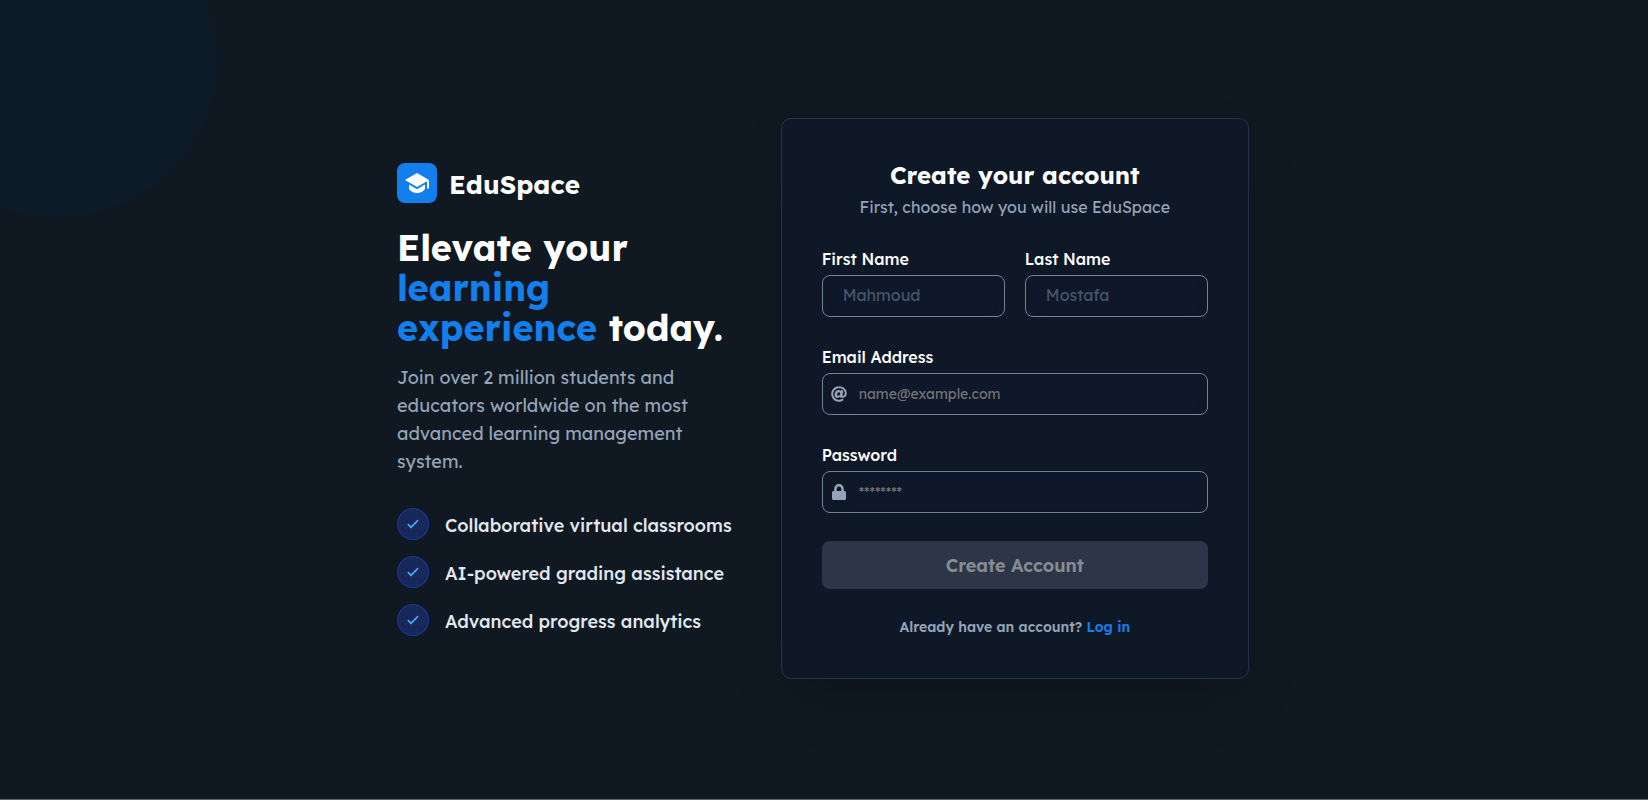
\includegraphics[width=\textwidth]{screenshots/register-page.png}
  \caption{Registration page with form fields for creating a new account.}
  \label{fig:ui-register}
\end{figure}

\begin{figure}[H]
  \centering
  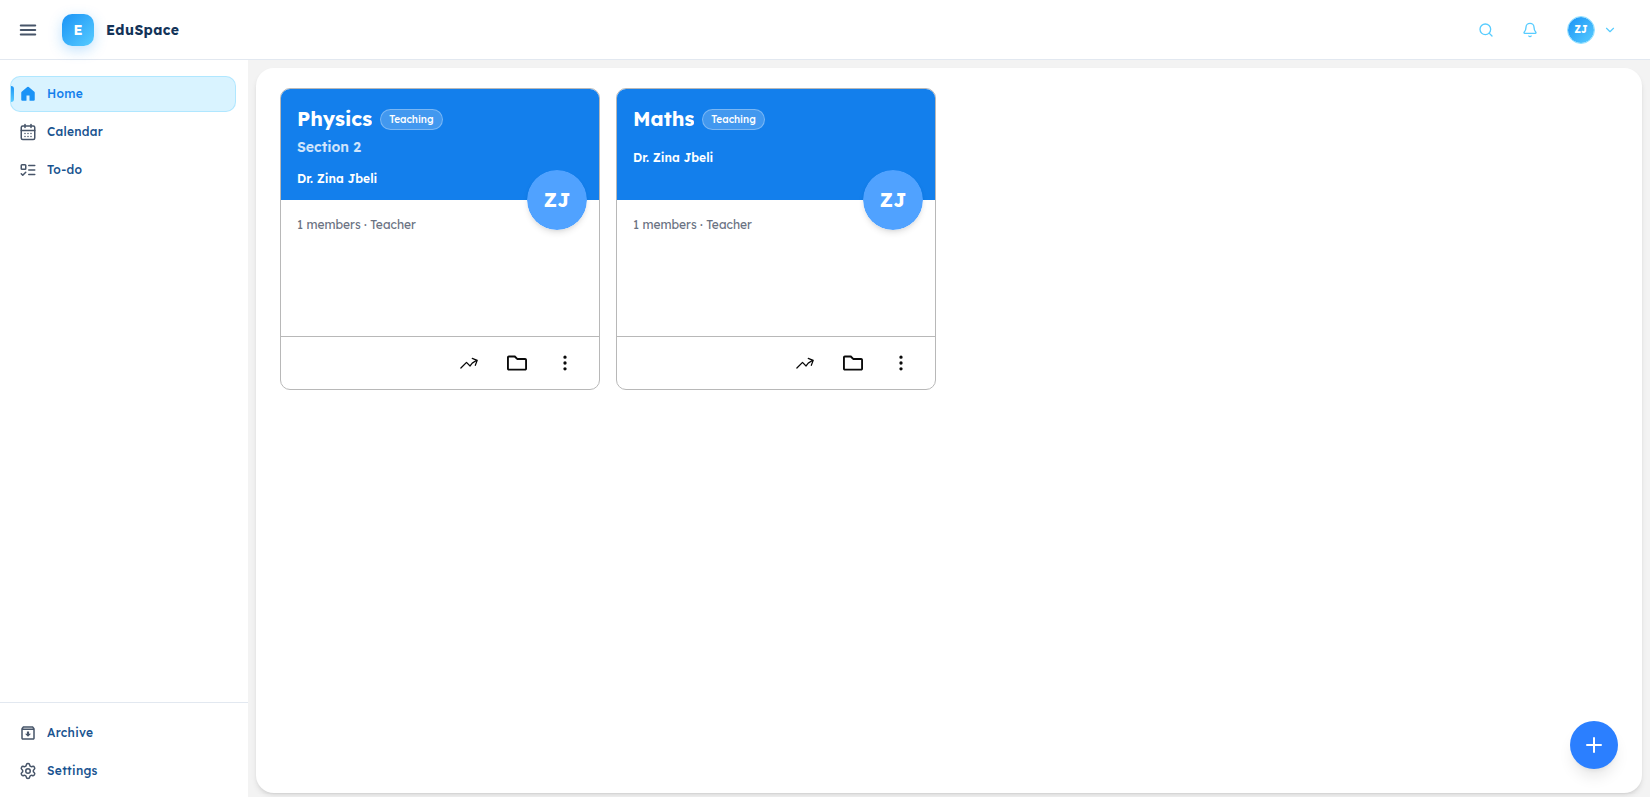
\includegraphics[width=\textwidth]{screenshots/dashboard.png}
  \caption{Dashboard showing classroom cards with type badges, member count, and quick actions.}
  \label{fig:ui-dashboard}
\end{figure}

\begin{figure}[H]
  \centering
  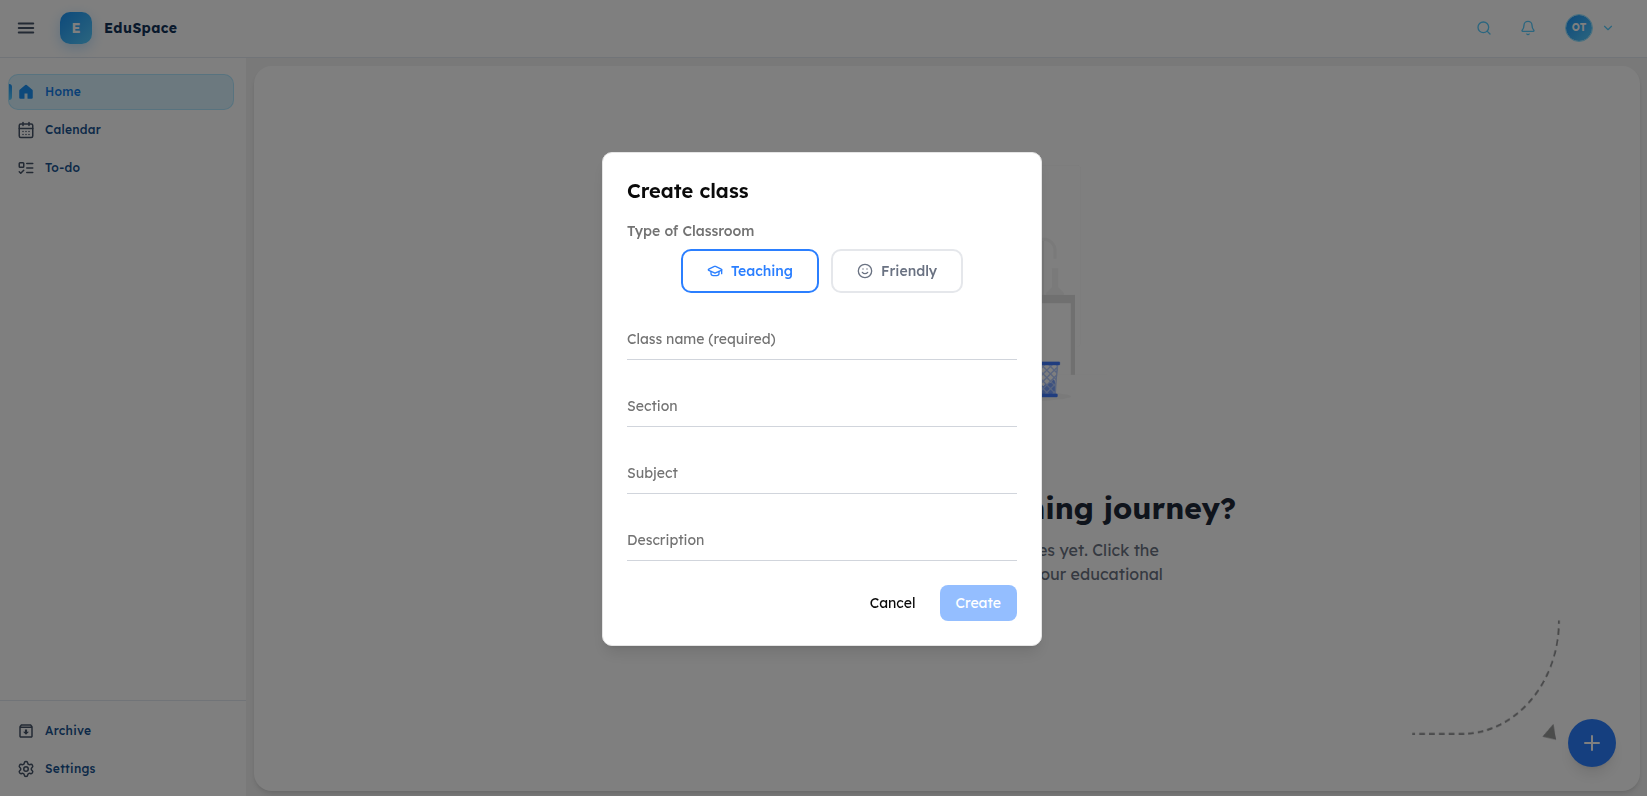
\includegraphics[width=0.55\textwidth]{screenshots/create-classroom.png}
  \caption{Create classroom dialog with name, type selection, and optional fields.}
  \label{fig:ui-create-class}
\end{figure}

\begin{figure}[H]
  \centering
  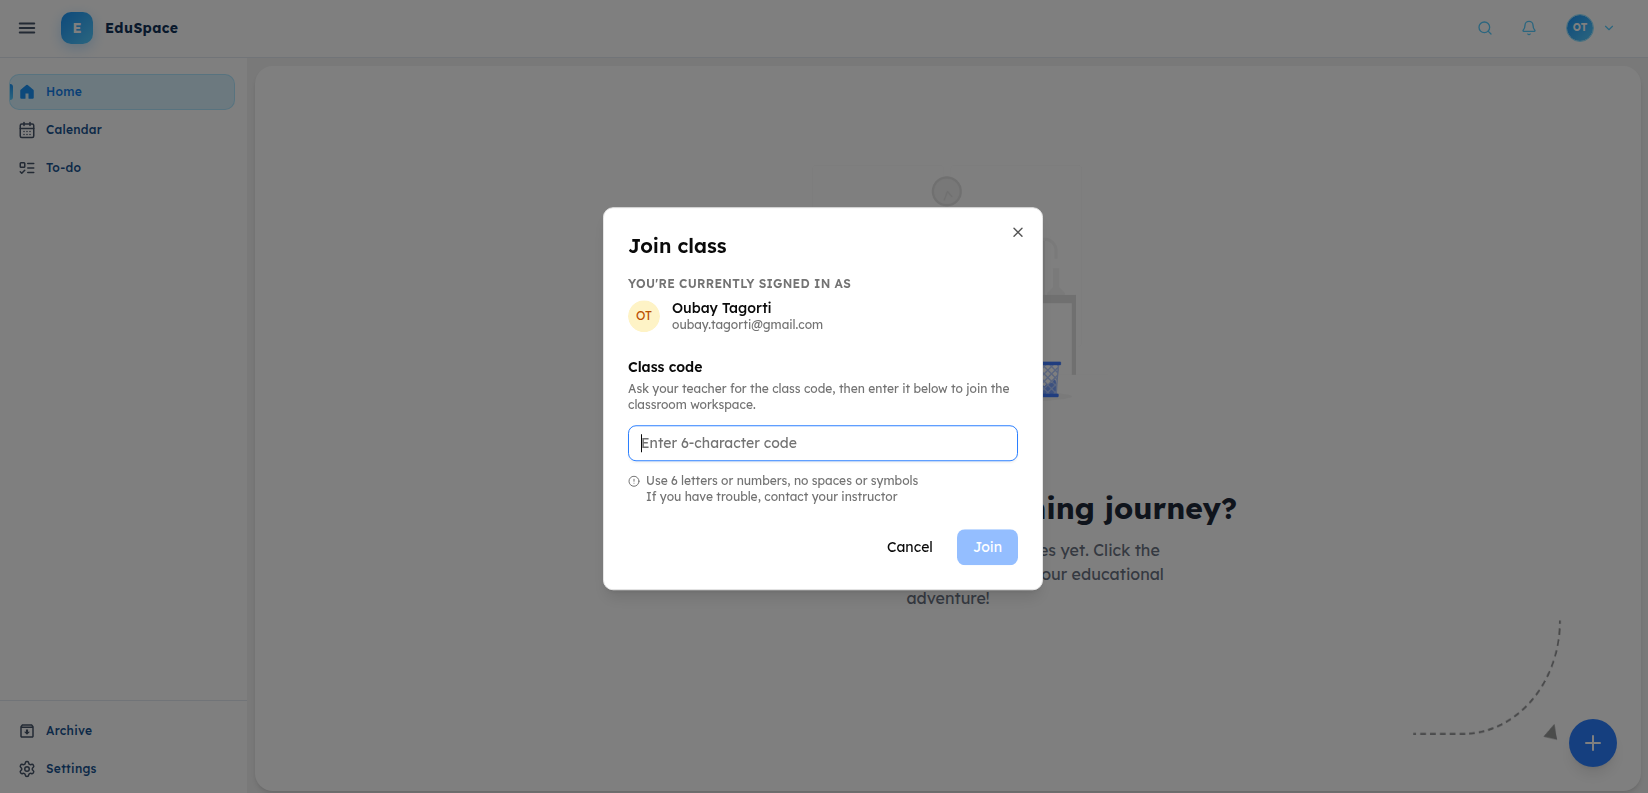
\includegraphics[width=0.55\textwidth]{screenshots/join-classroom.png}
  \caption{Join classroom dialog where users enter a 6-character class code.}
  \label{fig:ui-join-class}
\end{figure}

\begin{figure}[H]
  \centering
  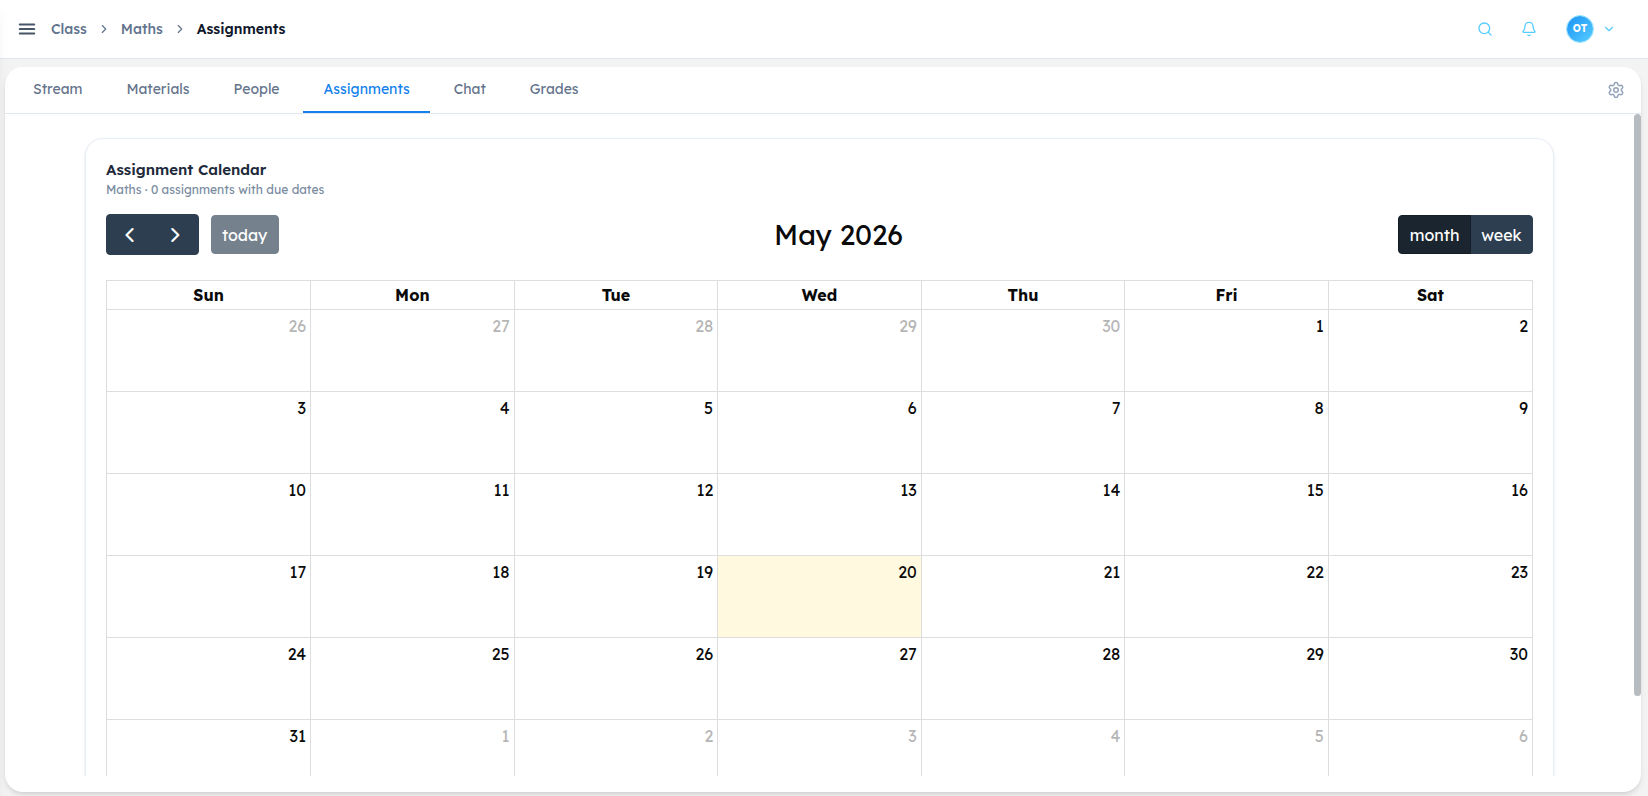
\includegraphics[width=\textwidth]{screenshots/assignments-tab.png}
  \caption{Materials tab displaying posts organized by chapter in an accordion layout.}
  \label{fig:ui-materials}
\end{figure}

\begin{figure}[H]
  \centering
  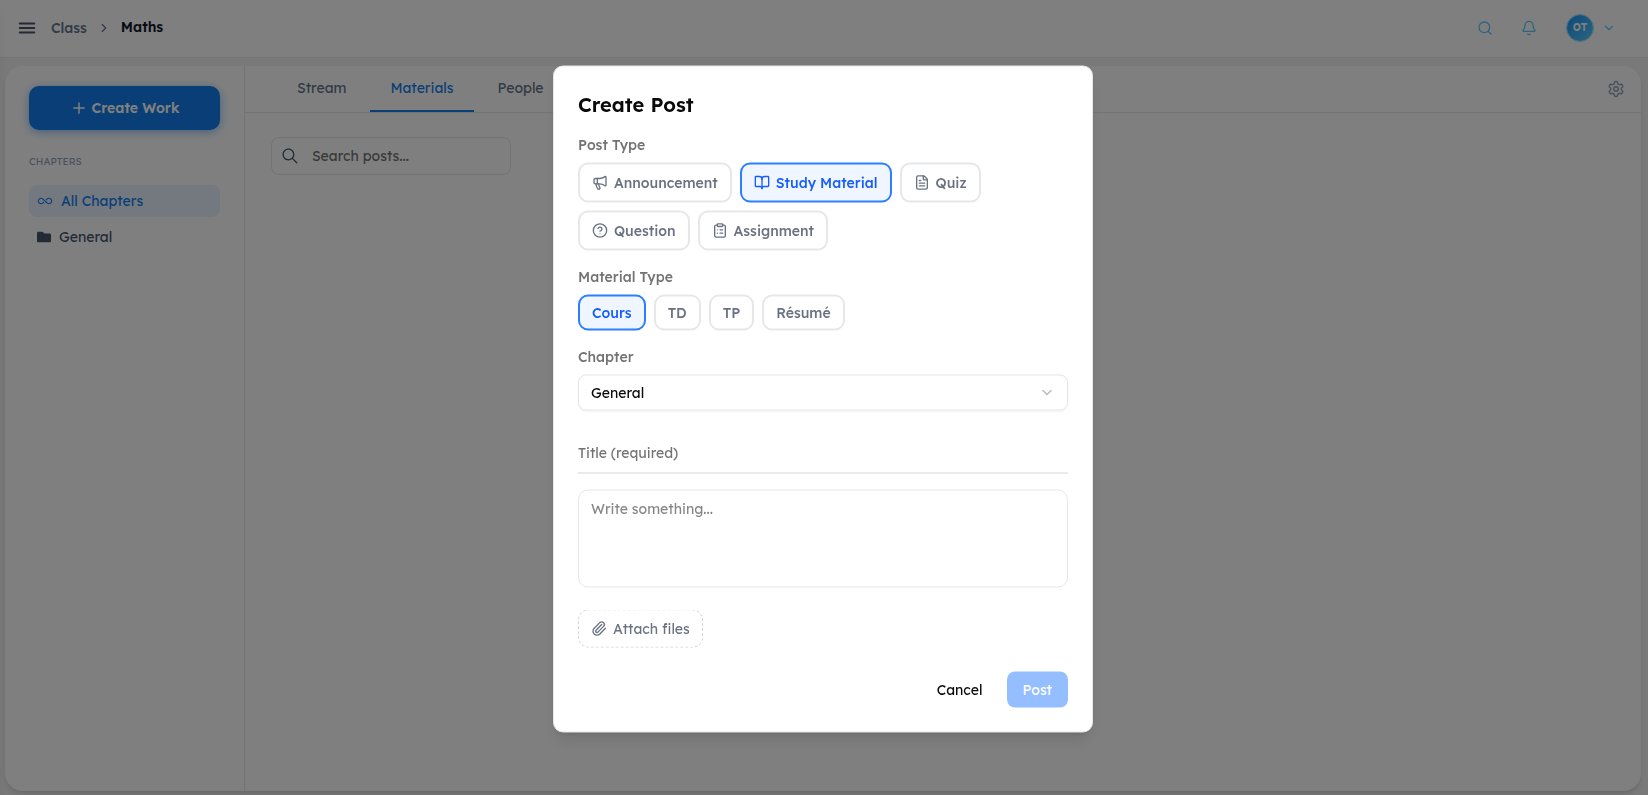
\includegraphics[width=0.6\textwidth]{screenshots/create-post.png}
  \caption{Post creation form with type selector, chapter assignment, and file attachments.}
  \label{fig:ui-create-post}
\end{figure}

\begin{figure}[H]
  \centering
  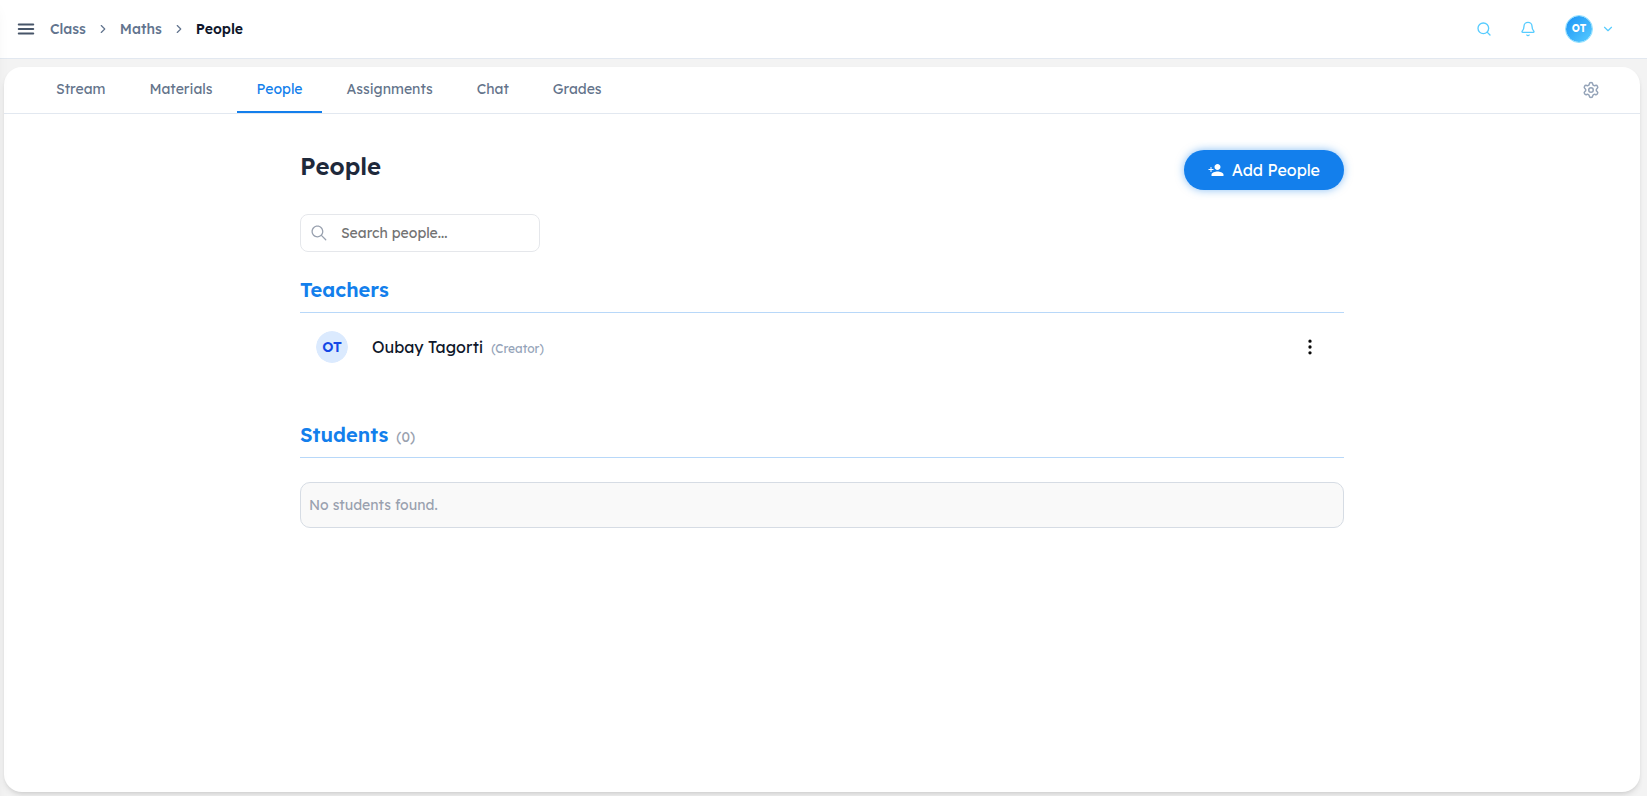
\includegraphics[width=\textwidth]{screenshots/people-tab.png}
  \caption{People tab listing classroom members grouped by role (Teachers and Students).}
  \label{fig:ui-people}
\end{figure}

\begin{figure}[H]
  \centering
  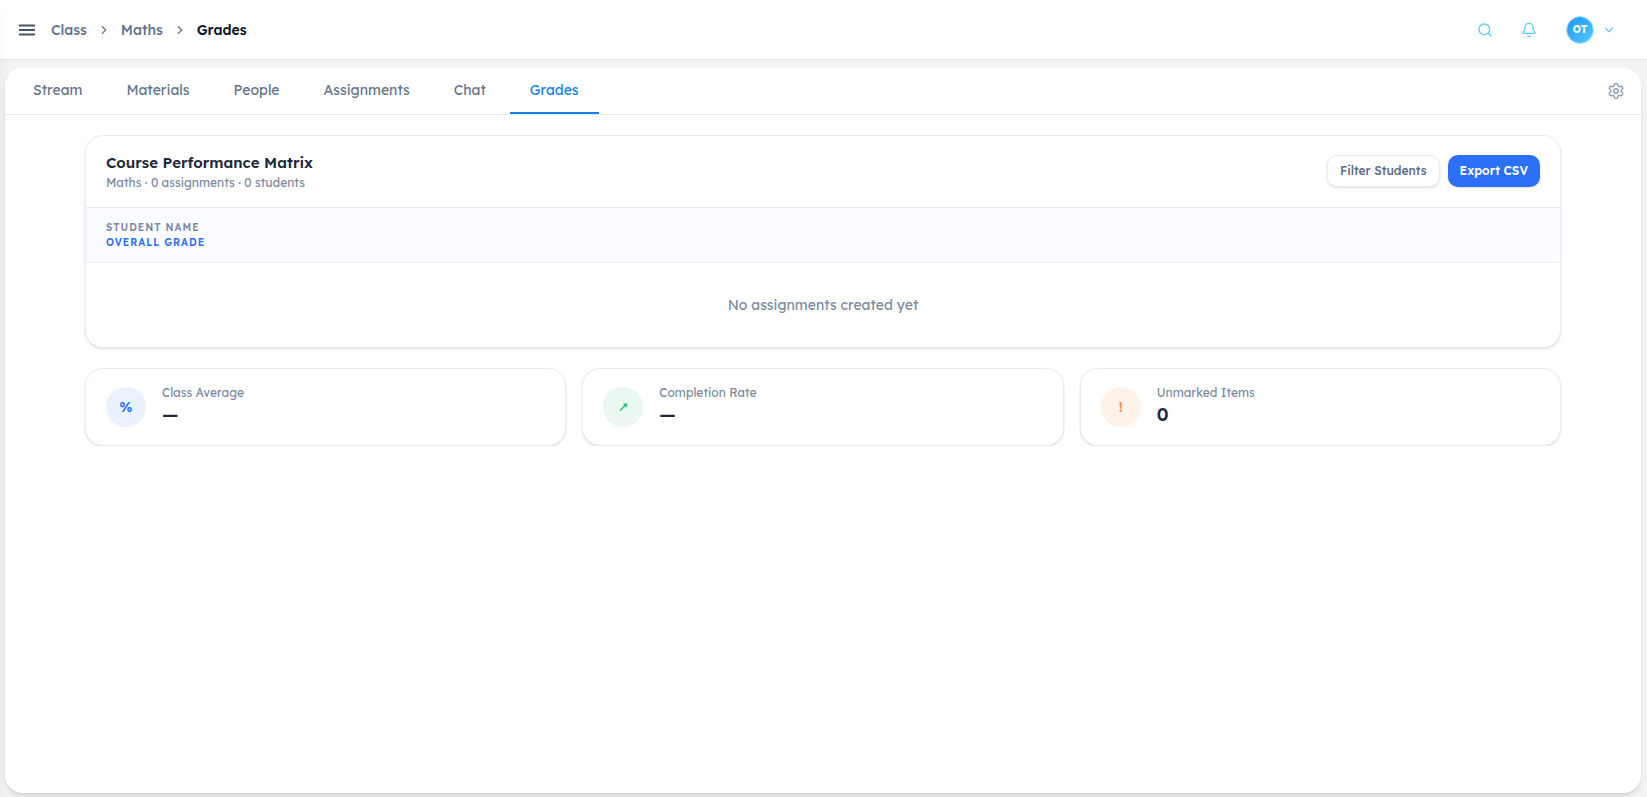
\includegraphics[width=\textwidth]{screenshots/grades-tab.png}
  \caption{Grades tab with the grade table showing assignments, scores, and averages.}
  \label{fig:ui-grades}
\end{figure}

\begin{figure}[H]
  \centering
  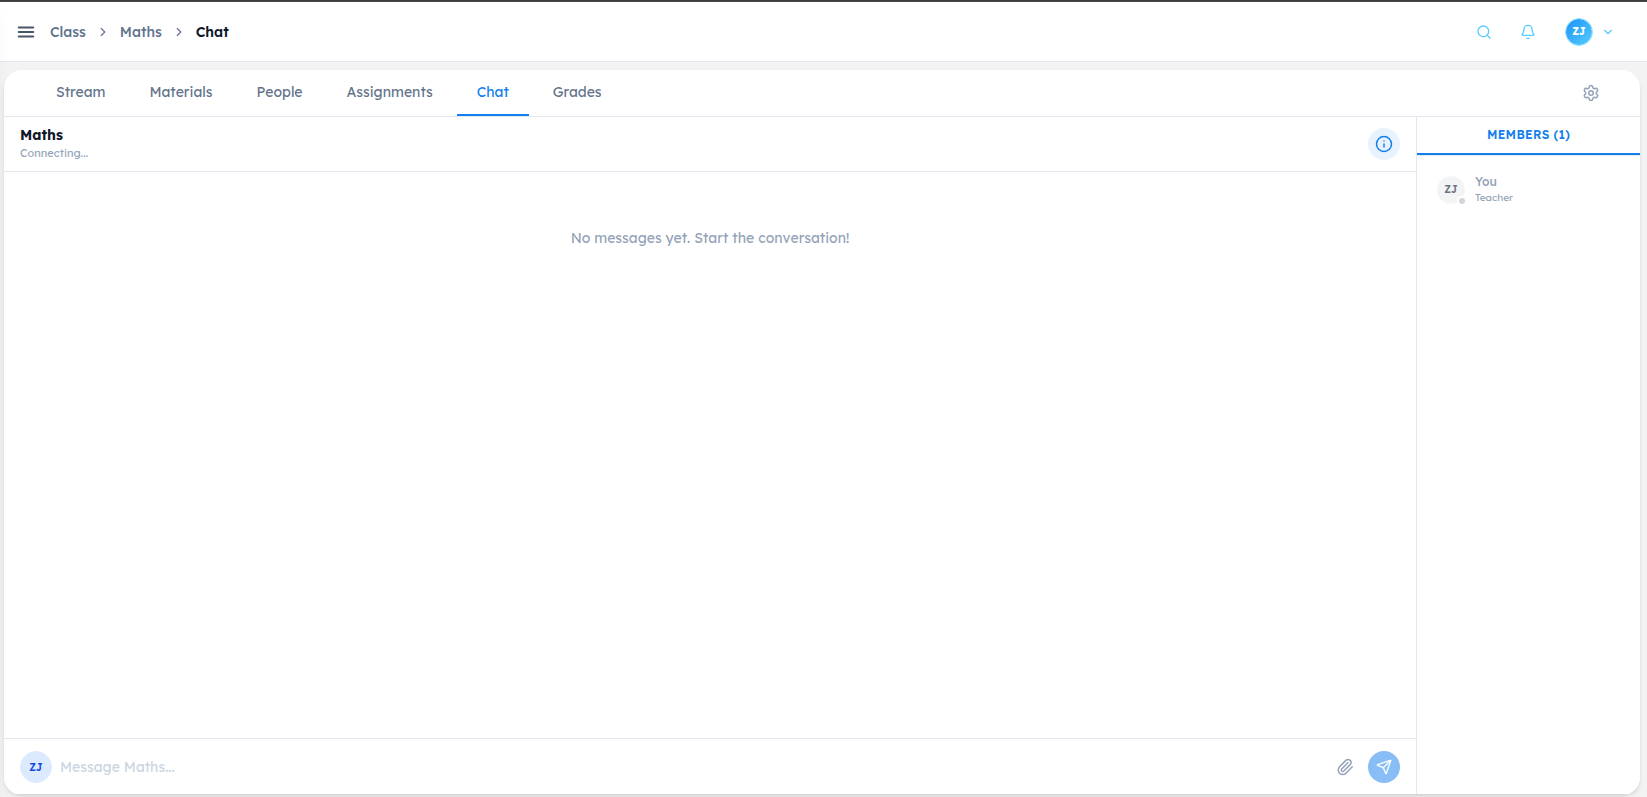
\includegraphics[width=\textwidth]{screenshots/chat-tab.png}
  \caption{Real-time group chat interface with message history and online indicators.}
  \label{fig:ui-chat}
\end{figure}

\begin{figure}[H]
  \centering
  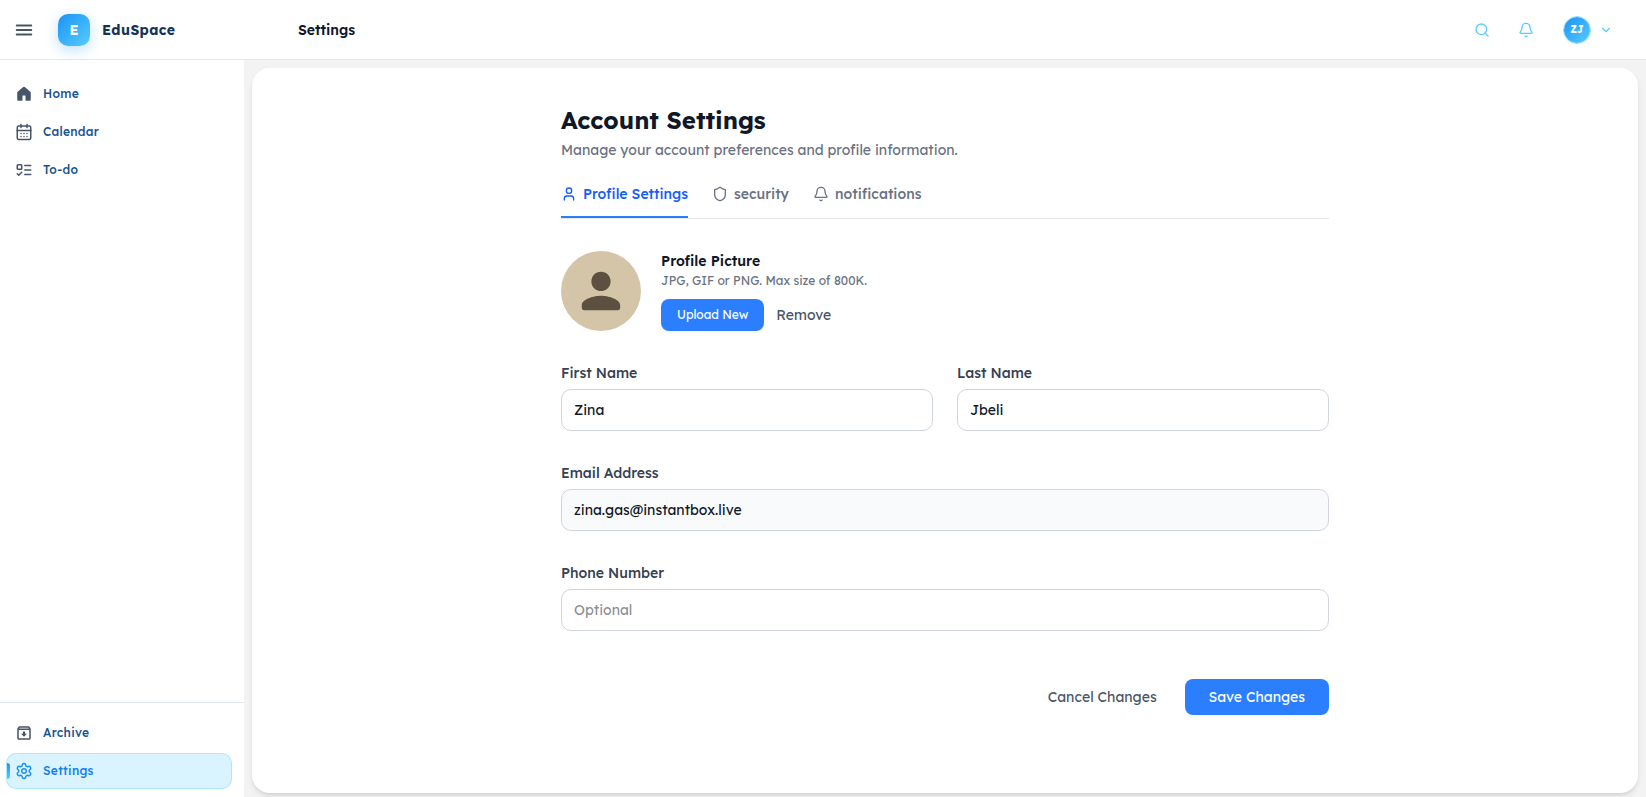
\includegraphics[width=\textwidth]{screenshots/account-settings.png}
  \caption{Account settings page for updating profile information.}
  \label{fig:ui-settings}
\end{figure}

\begin{figure}[H]
  \centering
  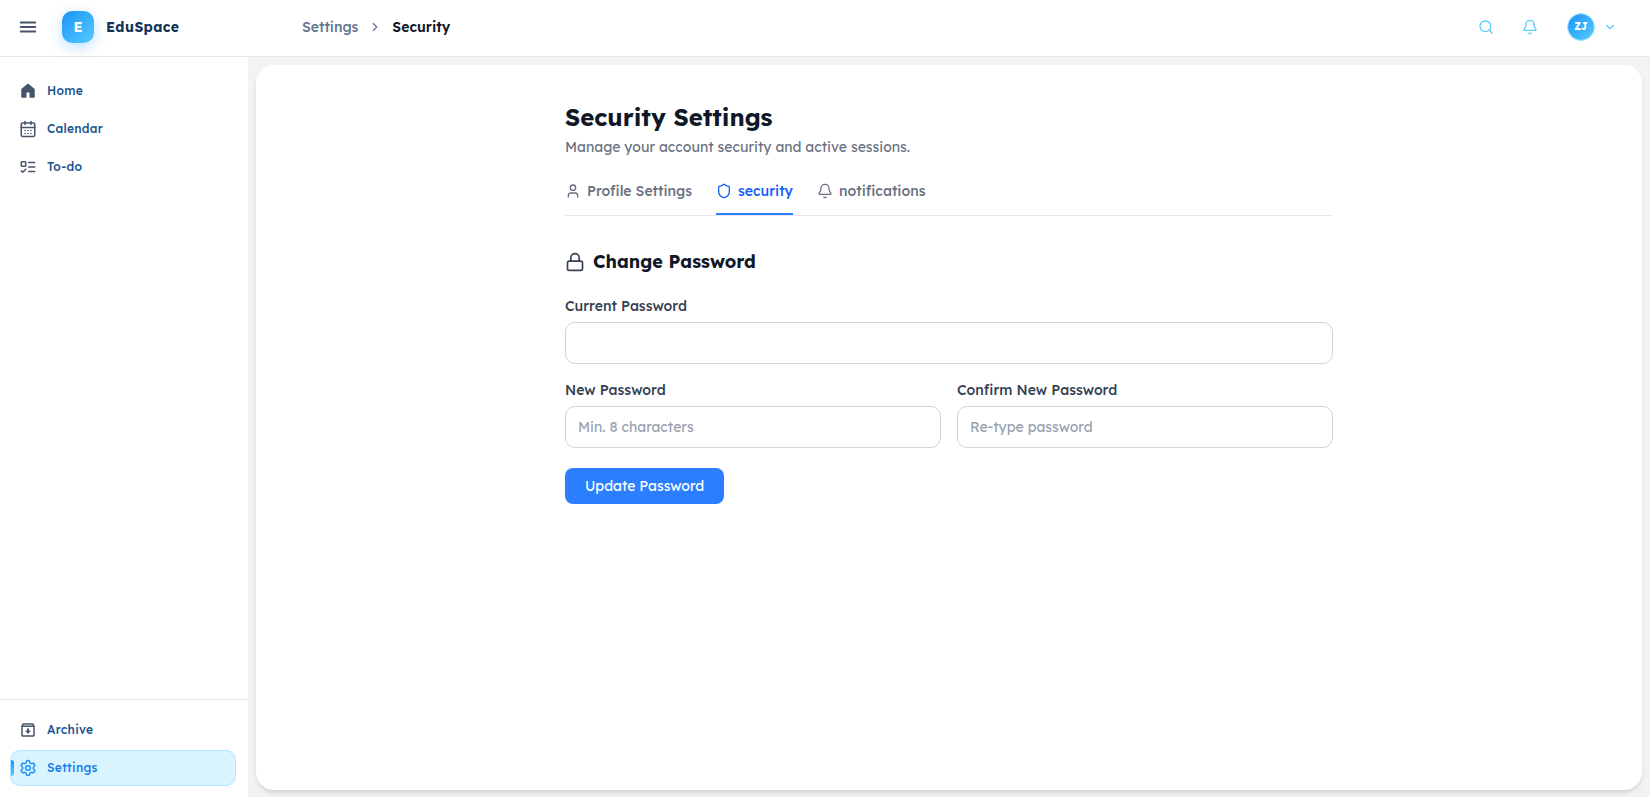
\includegraphics[width=\textwidth]{screenshots/security-settings.png}
  \caption{Security settings page for changing password.}
  \label{fig:ui-security}
\end{figure}

% =============================================================================
\section*{Conclusion}

This chapter detailed the implementation and deployment of \eduspace{}.
The technological framework was presented comprehensively, covering the frontend stack (React~19, TypeScript, Tailwind~CSS, TanStack libraries, FullCalendar, Socket.IO), the backend stack (Node.js, Express~5, Prisma, JWT, RabbitMQ, Redis), and the containerized infrastructure (PostgreSQL, Redis, RabbitMQ, MinIO, Elasticsearch, NGINX).
The development workflow, anchored by Git and GitHub with a feature-branch strategy, was described alongside the pnpm-based monorepo management and Prisma migrations.

Security was addressed as a layered concern---from NGINX and API Gateway-level protections through service-level authorization (role checks, membership verification, classroom type enforcement) to data-level safeguards (bcrypt hashing, presigned URLs, hashed reset tokens).

% General Conclusion and Perspectives
% =============================================================================
% General Conclusion and Perspectives
% =============================================================================
\chapter*{General Conclusion and Perspectives}
\addcontentsline{toc}{chapter}{General Conclusion and Perspectives}
\markboth{General Conclusion and Perspectives}{}

\section*{Results Achieved}

This project set out to design and implement \eduspace{}, a web-based classroom management platform that addresses the organizational and communicational shortcomings of existing solutions such as Google Classroom, Moodle, and Microsoft Teams for Education.

The platform was delivered as a fully functional system comprising:

\begin{itemize}[nosep]
  \item A \textbf{microservices backend} with seven independent services (User, Class, Content, File, Communication, Notification, Search) and an API Gateway, each owning its own data store and communicating through REST and RabbitMQ.
  \item A \textbf{React single-page application} providing a modern, responsive interface for authentication, classroom management, content browsing with filtering and sorting, real-time group chat, assignment submission and grading, a notification center, and full-text search.
  \item A \textbf{containerized infrastructure} orchestrated by Docker Compose, integrating PostgreSQL (five databases), Redis, RabbitMQ, MinIO, Elasticsearch, and NGINX.
\end{itemize}

\section*{Challenges Encountered}

Several technical challenges arose during development:

\begin{itemize}[nosep]
  \item \textbf{WebSocket authentication.}
        Integrating JWT-based authentication with Socket.IO connections required handling the token during the handshake phase rather than through standard HTTP headers, which differed from the REST authentication flow.
  \item \textbf{Elasticsearch indexing synchronization.}
        Keeping the search index consistent with the content database required reliable event publishing and idempotent consumers to handle message redelivery scenarios.
  \item \textbf{Monorepo dependency management.}
        Managing shared code across nine workspace packages while keeping dependency versions aligned demanded disciplined use of pnpm workspaces and a well-structured shared package.
\end{itemize}

\section*{Personal Contributions}

This project provided valuable hands-on experience in:

\begin{itemize}[nosep]
  \item Designing and implementing a distributed microservices architecture from scratch.
  \item Working with message brokers (RabbitMQ) for asynchronous inter-service communication.
  \item Integrating multiple infrastructure components (PostgreSQL, Redis, Elasticsearch, MinIO) within a containerized environment.
  \item Building a complete full-stack application with React, TypeScript, and modern frontend libraries (TanStack Query, Socket.IO, FullCalendar).
  \item Applying software engineering principles---requirements analysis, UML modeling, design patterns, and iterative development---to a real-world project.
\end{itemize}

\section*{Future Perspectives}

Several enhancements could extend \eduspace{} beyond its current scope:

\begin{itemize}[nosep]
  \item \textbf{Video conferencing.}
        Integrating WebRTC-based video calls directly within classrooms would eliminate the need for external tools for synchronous lectures.
  \item \textbf{Mobile application.}
        A native mobile client (React Native or Flutter) would improve accessibility for students who primarily use smartphones.
  \item \textbf{AI-powered features.}
        Automatic quiz generation from study materials, plagiarism detection on submissions, and intelligent content recommendations could enhance the learning experience.
  \item \textbf{Analytics dashboard.}
        Providing instructors with engagement metrics (post views, submission rates, chat activity) would enable data-driven teaching adjustments.
  \item \textbf{Kubernetes deployment.}
        Migrating from Docker Compose to Kubernetes would enable horizontal scaling, self-healing, and production-grade orchestration for larger deployments.
  \item \textbf{OAuth and SSO.}
        Supporting third-party authentication providers (Google, Microsoft) would simplify onboarding for institutions already using these ecosystems.
\end{itemize}


% ── References ───────────────────────────────────────────────────────────────
\printbibliography[heading=bibintoc, title={References}]

\end{document}
